% !TEX encoding = UTF-8 Unicode

\documentclass[12pt,a4j]{ltjsarticle}
\usepackage{semi}
\usepackage{here}

%\title{個人でのVR技術の利用状況} 
%\author{三原巧巳}
%\date{2022年12月14日} 
\begin{document} 

\begin{titlepage}
 \begin{center}
  
    \vspace*{20truept}
    
    {\LARGE 2022年度 卒業論文} 
    
    \vspace*{75truept}
    
    {\LARGE 個人でのVR技術の利用状況}
    
    %{\Huge } 個人でのVR技術の利用状況
    
    \vspace{85truept}
    
    {\LARGE 指導教員 須田 宇宙 准教授}
    
    \vspace{60truept}
    
    {\LARGE 千葉工業大学 情報ネットワーク学科}
    
    \vspace{15truept}
    
    {\LARGE 須田研究室}
    
    \vspace{70truept}
    
    {\LARGE 1931131 氏名 三原 巧巳 } % 氏名は消さない 学生番号 氏名 名前

    \vspace{70truept}
    
  \end{center}
  \begin{flushright}

    {\LARGE 提出日 2023年1月17日}
  
  \end{flushright}
\end{titlepage}
\clearpage

\setcounter{tocdepth}{3}
% 目次の出力
\tableofcontents
% 表目次
%\listoftables
% 図目次
\listoffigures
\clearpage
\pagenumbering{arabic}
\setcounter{page}{1}

%\clearpage

%\tableofcontents
%\clearpage

\section{緒言}
近年,xR(AR,MR,VR)技術の発展により日常生活で技術の使用やコンテンツを見かけることが多くなった.
現在,xR技術は様々な形に変化して利用されている.
AR技術を利用するにはスマートフォンやスマートグラス,MR技術を利用するにはメガネや大きな機械のカメラなどで利用されている.
この2つの技術を用いたコンテンツは,広いスペースや大掛かりな設備を必要としない.

一方,VR技術を利用するには専用のヘッドマウントディスプレイを頭に着用し,視界の全体を覆った上で動き回るため,利用するコンテンツによっては大きな機材や広いスペースを必要とすることがある.
VR技術は主にゲームやアトラクション施設の場で利用されることが多いが,実際に利用できる施設や利用する場面が少ない.
利用される機会が少ないことで,VR技術の普及が低く技術の進化が起こらなくなる.
VR技術の進化がされないことで起こってしまうことは,エンターテイメントの幅が広がらないだけだはなく,現実で行うには危険な実習や現実では起こしにくい体験をすることが困難になるという問題がある.

本研究では,VR技術が普及しない理由として,現在あるVR技術のコンテンツにあると仮説を立て,それを元にVR機器の普及度と,購入されている種類・傾向,および購入していない人に対して購入していない理由などについて調査をし,普及率が低い原因を見つけることを目的としている.
\clearpage

\section{xR技術について}
\subsection{VR技術}
\subsubsection{VR技術とは}
VRとは,「Virtual Reality」の略称であり「仮想現実」とも呼ばれている.
VR専用のヘッドマウントディスプレイやVRゴーグルを装着して,視界全体にコンピューターで作成した空間や世界の映像を映すことで自分が映像の中に入り込んだような体験ができる技術である.
さらにVRの中で自由な移動やものの操作などができ,現実に近い体験から非現実的な体験まで幅広くが扱うことができる.

VRコンテンツを利用するためには,専用のゴーグルが必要になりコンテンツによっては専用のコントローラーなども必要となる.
また体を動かすコンテンツの場合動かすのに十分な空間も必要となる.

VRのコンテンツには,現実世界を360°のカメラで撮影し動画や静止画として編集した実写VRコンテンツとCG技術を利用して仮想世界や現実ではあり得ない映像を表現するCGVRコンテンツの2種類がある.
実写VRコンテンツは主に観光PRやライブの映像,教育や研修などのコンテンツが存在し,CGコンテンツはゲームなどのコンテンツが存在する.

VR技術では,主にゲームやエンターテイメントで普及してきたが,幅広い体験をできることから教育や訓練などでも利用されるようになり,近年ではビジネスの分野でも活躍するようになっっている.
ゲームやエンターテイメントの場では,専用のヘッドマウントディスプレイを利用したゲームの世界観を体験しながら遊べるコンテンツがある.
教育や訓練の場では,VRを利用した社会科見学や避難訓練の再現などといったもので利用されている.
ビジネスの場では,VRでの物件の内見やVRでのショッピングなどといったサービスが増えていっている.

\subsubsection{VR技術の歴史}
VR技術のコンセプトは1935年ごろに作家のスタンリー・G・ワインボウムが発表したSF短編小説
「Pygmalion's Spectacles」の中に,ゴーグルを装着すると仮想的に五感を感じ取りながら擬似体験が可能な装置が登場する.

VR技術の研究が始まったのは1960年代前後からである.映画作成者で仮想現実技術のパイオニアであるモートン・ヘイリグが1957年にセンソラマと呼ばれる世界最初期のVR機器が開発された.
センソラマとは図\ref{fig:センソラマ.pdf}のような大型のシステムであり,没入型で多感覚入力が可能というマルチモーダルインターフェースを採用している.

\begin{figure}[h]
\begin{center}
 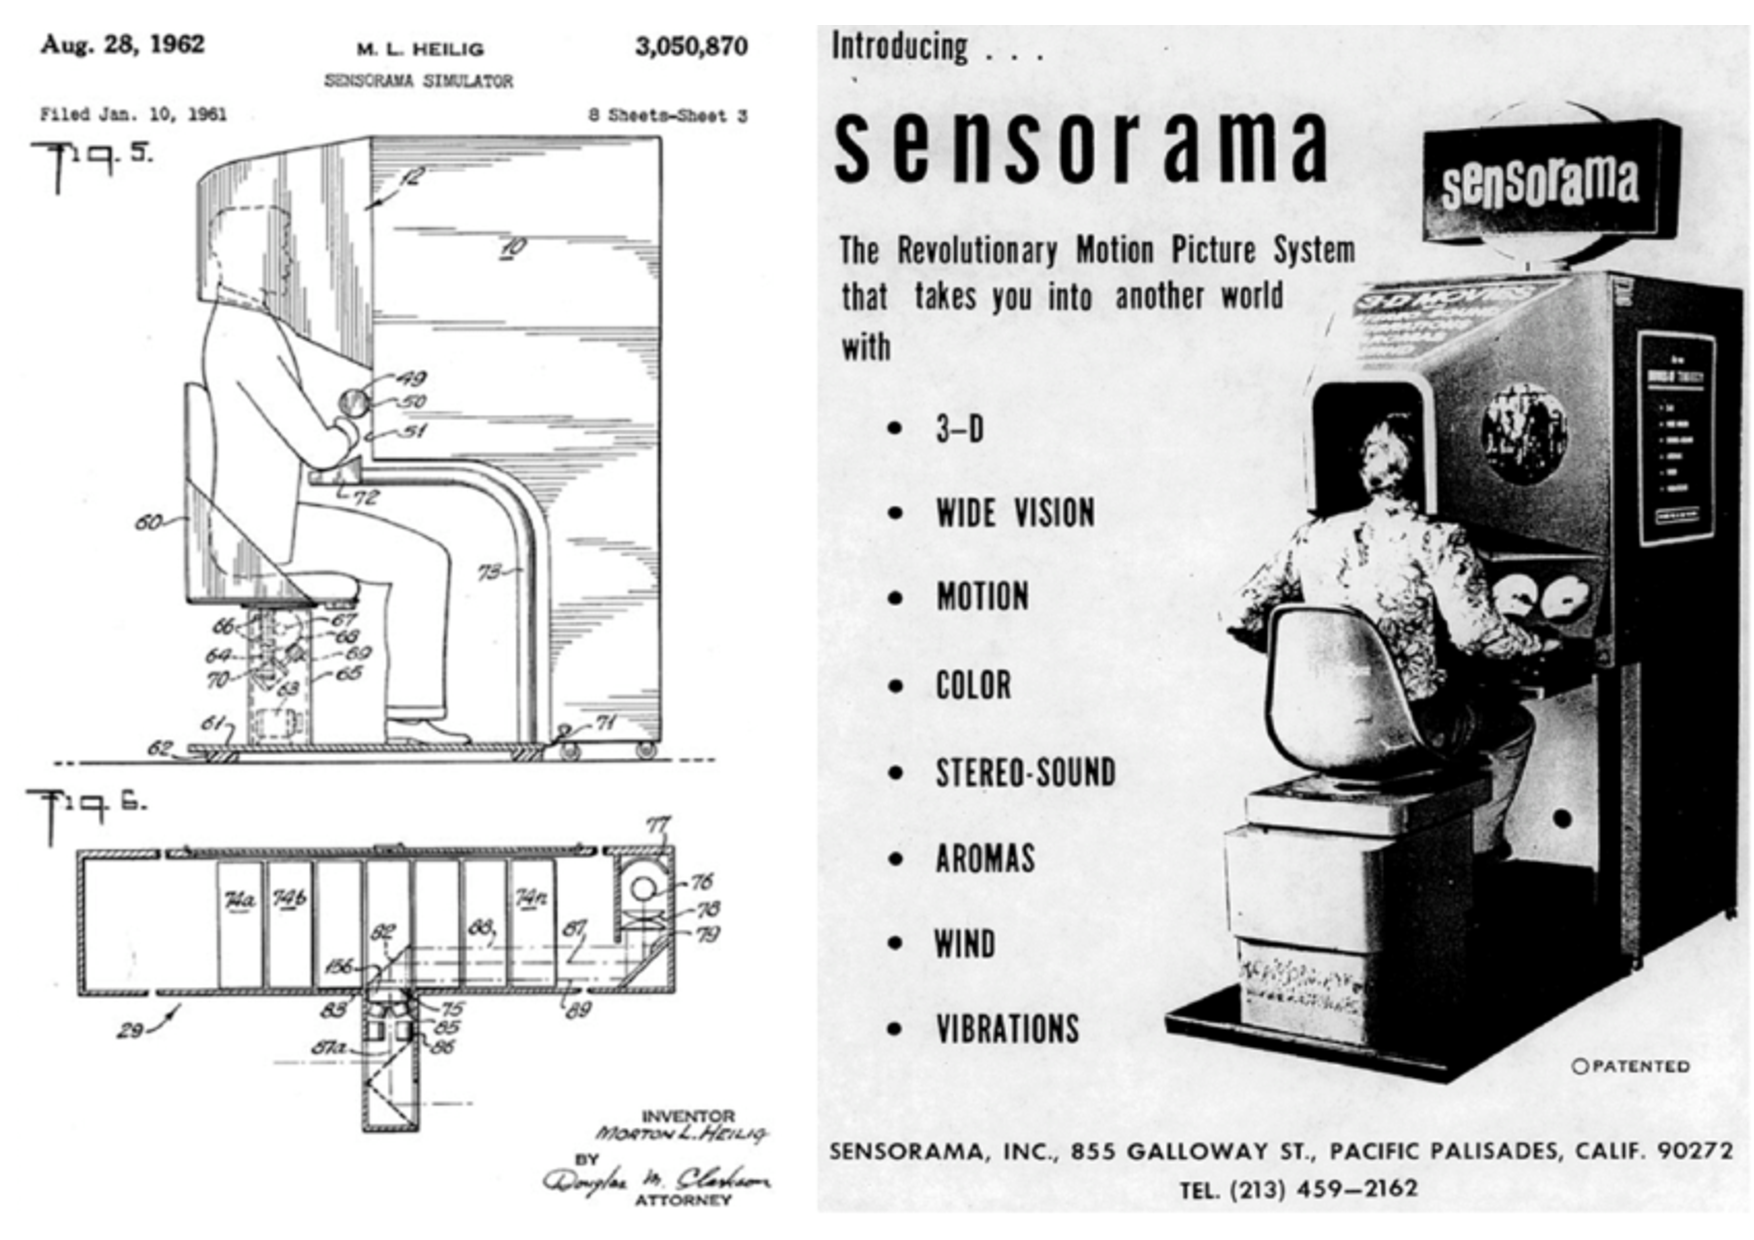
\includegraphics[clip,height=55mm]{センソラマ.pdf}
\end{center}
 \caption{センソラマ}
 \label{fig:センソラマ.pdf}
\end{figure}

その後1968年にユタ大学のアイバン・サザランドは,「ダモクレスの剣」というヘッドマウントディスプレイを開発したが,どちらも実用性が低くかった\cite{VRの概念の登場}.

1990年代前後からVR機器の商用化が始まった.
VPL Research社がRB2(Reality Built dfor 2)というVRを利用したコミュニケーションシステムを発表した.
このシステムは,ヘッドマウントディスプレイを使用した2人が同じVR空間で会話ができる3Dテレビ会議のようなシステムのようなシステムである.
しかし,当時のVR機器は価格が高いだけではなく性能が価格と見合っていないということから一般家庭に普及しなかった.
この商用化から約10年間はVRの第1次ブームと言われている\cite{VRの初の商用化}.

スマートフォンやゲーム機などのハードウェアの進化により2010年代以降にVRが再び注目される\cite{VRの概念の登場}.
スマートフォンでVRを利用したアプリケーションが開発されたり,以前より安価で性能が高くなった機器が出たことから,第1次ブームの時よりも日常的なものになろうとしている.

\subsection{AR技術}
\subsubsection{AR技術とは}
ARとは,「Augmented Reality」の略称であり「拡張現実」とも呼ばれており,現実を仮想的に拡張する技術である.
具体的にはスマートフォンやタブレットなどのカメラを通して現実世界を映し,その上にCG映像や文字情報を重ねることで重ねたデータが実在しているように見える技術である\cite{ARとは}.

ARコンテンツを利用するためには,専用の機材を必要とせずスマートフォンやカメラがついているPCなどで利用することができる.

AR技術は,元々PCで利用されていた技術だったかスマートフォンの技術が進歩したことにより気軽に利用できる技術になった.
スマートフォンで利用できるようになったためエンターテイメントの分野でも活躍するようになった.

\subsubsection{AR技術の歴史}
現在のAR技術の概念の登場は1901年である.
小説家のライマン・フランク・ボームが書いた「The Master Key: An Electrical Fairy Tale」の中で登場した現実の世界にデジタルを重ね合わせる電子ディスプレイの概念を提唱したことが始まりとされている.

1968年にハーバード大学教授であり計算機科学者であったアイバン・サザランドが教え子のボブ・スプロールと共に仮想現実を創り出すヘッドマウントディスプレイ・システム「The Sword of Damocles」を開発した.

\begin{figure}[h]
\begin{center}
 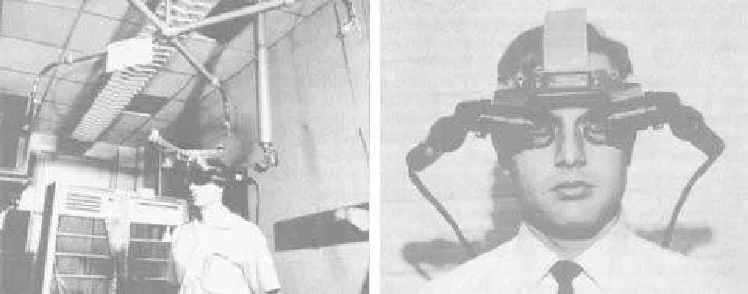
\includegraphics[clip,height=55mm]{The_Sword_of_Damocles.pdf}
\end{center}
 \caption{The Sword of Damocles}
 \label{fig:The_Sword_of_Damocles.pdf}
\end{figure}

図\ref{fig:The_Sword_of_Damocles.pdf}のデバイスを装着することで,ユーザーはCGで作られた環境で仮想体験ができるというシステムである.
しかしこのデバイスは重すぎるため天井から吊り下げて使用するというものになっている.
また,仮想空間で作り出せるものはシンプルな線のみでの構成になっている.

1973年にAR技術は,「Augmented Reality」の前に「Artificial Reality」または「人工現実」として提唱されていた.
この技術はAR技術ではなくVR技術に近いものである.
「Augmented Reality」は1990年にトム・コーデルが名付けた.

1990年代にITによる効率化の影響によりAR技術は急速に進化していった.
1992年にアメリカ空軍で世界初の操作可能のARシステムが開発された.
このシステムは現在のAR技術が持つ基本性能を持っているとされている.
1993年にコロンビア大学のスティーブン・フェイナーがレーザープリンターのメンテナンスのサポートを行うARシステムを発表した.
このシステムはHMDを装着することで,超音波センサーにより検知したレーザープリンターの内部構造情報や修理が必要な箇所がコンピュータグラフィックで表示することができた.
しかし,このシステムは対象物に超音波センサをつけなければいけなかったため実用化はされなかったが,現在の業務用ARシステムのコンセプトを作り出したシステムとなっている.
ここからAR技術は舞台やテレビ,飛行機などにも利用されるようになり急成長していった.

1999年にARアプリケーションを実現するためのライブラリ『ARToolKit』が,当時ワシントン大学HITラボ滞在中だった奈良先端科学技術大学院大学の加藤博一によって高度技術の研究用のC言語ライブラリとして開発された.
1990年代のシステムは高価な位置姿勢計測装置が必要だったが,「単眼カメラ」と「平面マーカー」のみを使って実装するARアプリケーションの開発を可能にしただけでなく,AR技術をより容易に使うことを可能にした.

2000年に入り,携帯端末の性能が向上したことにより様々なARのアプリケーションが誕生し一般に広まった.
2013年にGoogleが発表した「Google Glass」の登場によりグラス型のデバイスが増えていった.
図\ref{fig:Google_Glass.pdf}のように手荷物必要のないハンドフリーかつスタンドアローン型の新しいパソコンとして期待されたが,社会問題と技術問題から一般的な販売は中止になった\cite{ARの歴史}.

\begin{figure}[h]
\begin{center}
 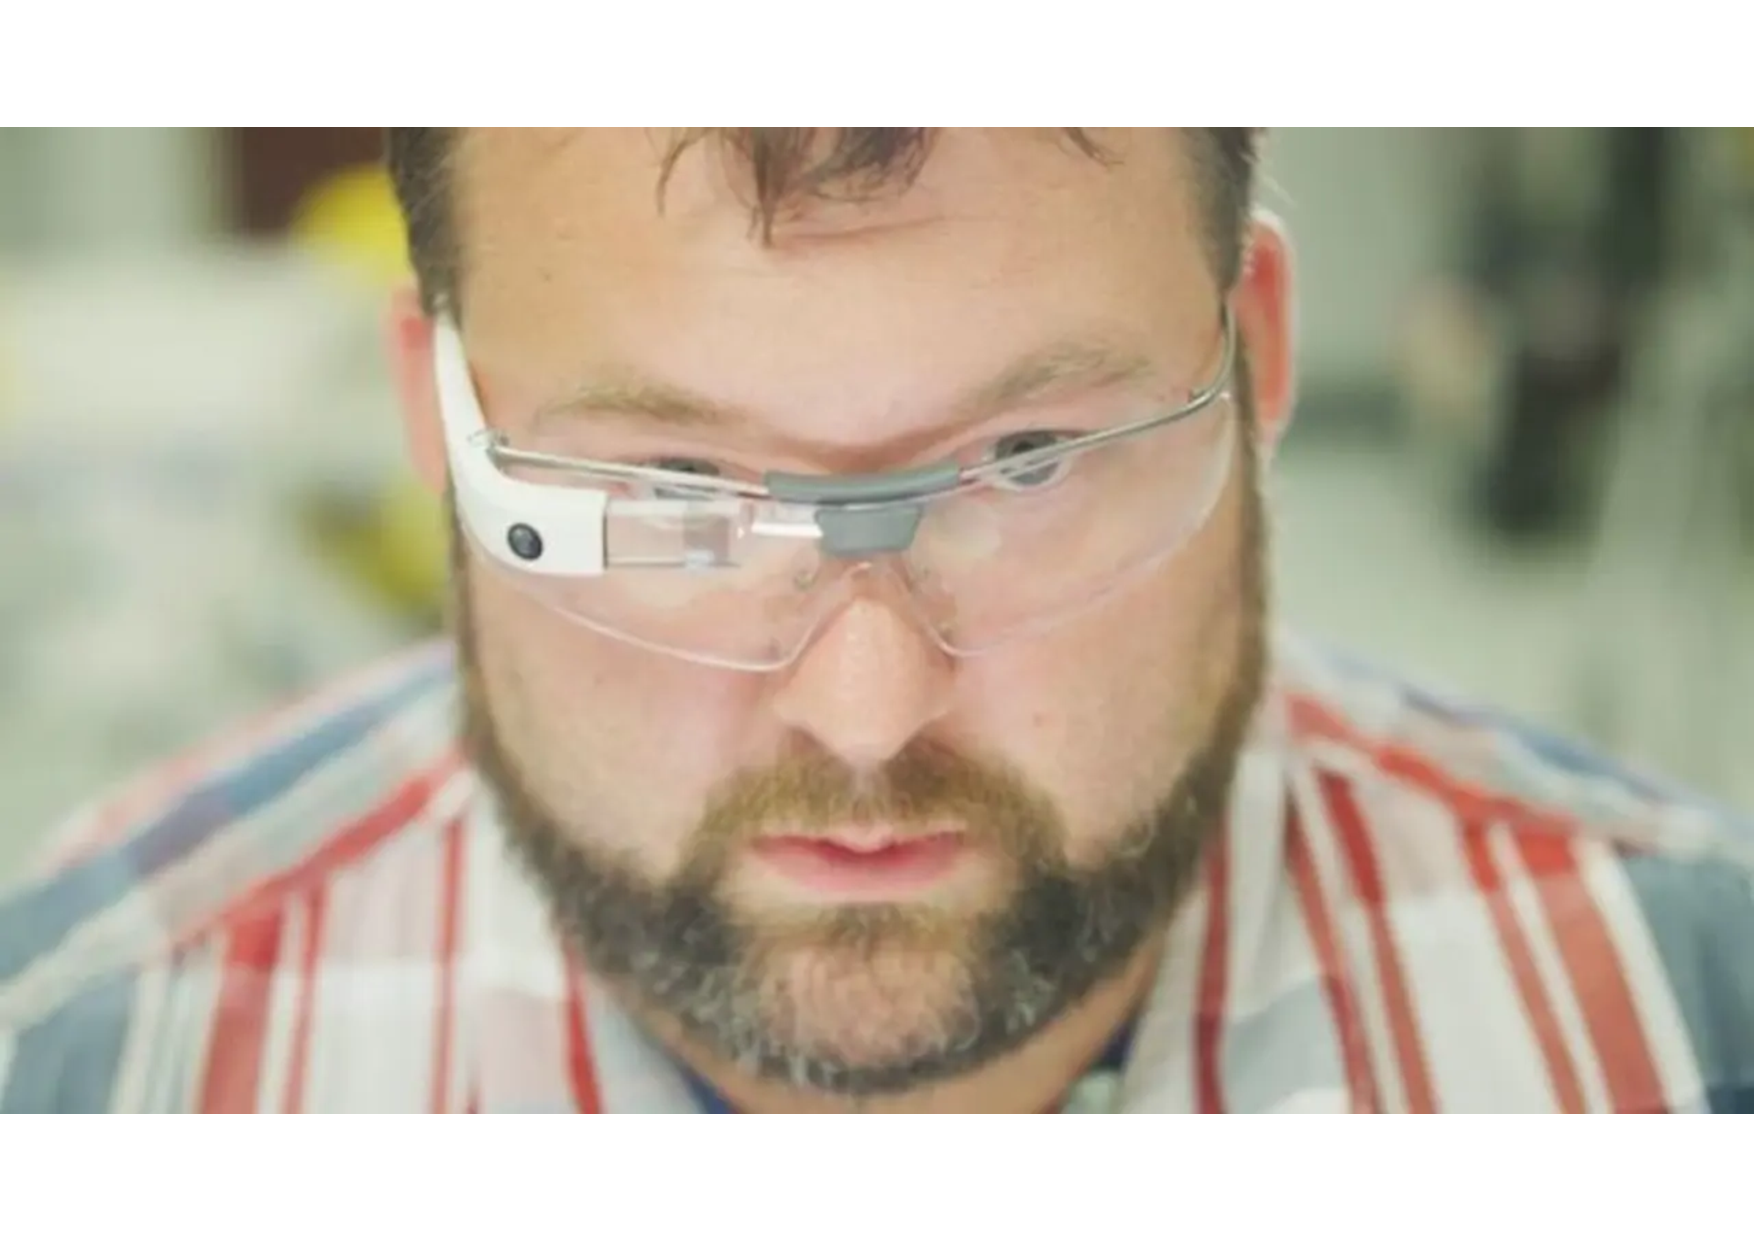
\includegraphics[clip,height=55mm]{Google_Glass.pdf}
\end{center}
 \caption{Google Glass}
 \label{fig:Google_Glass.pdf}
\end{figure}

\subsection{MR技術}
\subsubsection{MR技術とは}
MRとは,「Mixed Reality」の略称であり「複合現実」とも呼ばれいる.
ヘッドマウントディスプレイやカメラで現実世界を認識し,そこに合わせたCG映像や文字情報などを重ねて表示することで現実世界と仮想世界を融合させる技術である.
MR技術では,現実世界の景色も見ることができるため仮想データを見ながら現実世界で体を移動させたり,仮想世界で作成したものを多角的に見ることが可能になる.
MR技術はAR技術と似ているが,AR技術は主体が現実世界でありそこに仮想データの情報だけを表示する技術であり,MR技術は現実世界と仮想世界の融合のため実際にそこにあるかのように現実とかそうが相互作用するようなリアルタイム映像の技術である\cite{MRとは}.

主にMR技術はビジネスの場で使われることが多く,建設現場の完成イメージの確認や研修の再現,医療現場での患者の情報表示などといった場で利用されている.

MR技術を利用するには,ヘッドマウントディスプレイやカメラだけではなく,コンテンツによっては仮想世界で作られたものを映すためのマーカーなども必要となる.

\subsubsection{MR技術の歴史}
MR技術は1994年にトロント大学のP.Milgramによって提唱された.
計算機内に構築される仮想世界と現実世界で強化するという概念を仮想化現実と呼び,現実世界を電子的に強化と増強することを拡張現実と対置した上で両方の要素を取り入れたMRを提唱した.
1997年に「複合現実感システムに関する試験研究」で複合現実感という言葉が登場した.
MR技術の研究は1993年ごろから始まっており,ヘッドマウントディスプレイによる情報提示を活用するという研究だった\cite{MRの歴史1}.

MR技術が市場に流通したのは2015年である.
発表されたものは,スタンドアローン型のヘッドマウントディスプレイで,コントローラーを必要とせずハンドトラッキングと音声入力で操作するものである.
この発表でMR技術は新たな体験をできる機材として市場に認知されるようになった\cite{MRの歴史2}.

その後,機器の軽量化や視線に応じて見ている映像が変化する技術,ホログラムで表示されたものを摘んだりする技術などによってより現実に馴染むことが可能になる機器が登場した.

現在市場に存在するMR機器は3種類のみであり,機器の独自性が高くなっている.

\clearpage
\section{xRの機材について}
\subsection{VRの機材}
VRの機材は1957年に図\ref{fig:センソラマ.pdf}の機材が初めてのVR機材である.
センソラマは筐体型の機材で,椅子に座り目の前にある巨大スクリーンで3D映像を見る装置である.匂いの生成や椅子の振動,送風などの機能が付いている\cite{VRの機材}.

1960年にTelsephere Maskが登場した.この機材は図\ref{fig:Telesphere_Mask.pdf}のようにヘッドマウントディスプレイでありセンソラマのように3D映像を見ることができるがモーショントラッキング機能は付いていない.

\begin{figure}[h]
\begin{center}
 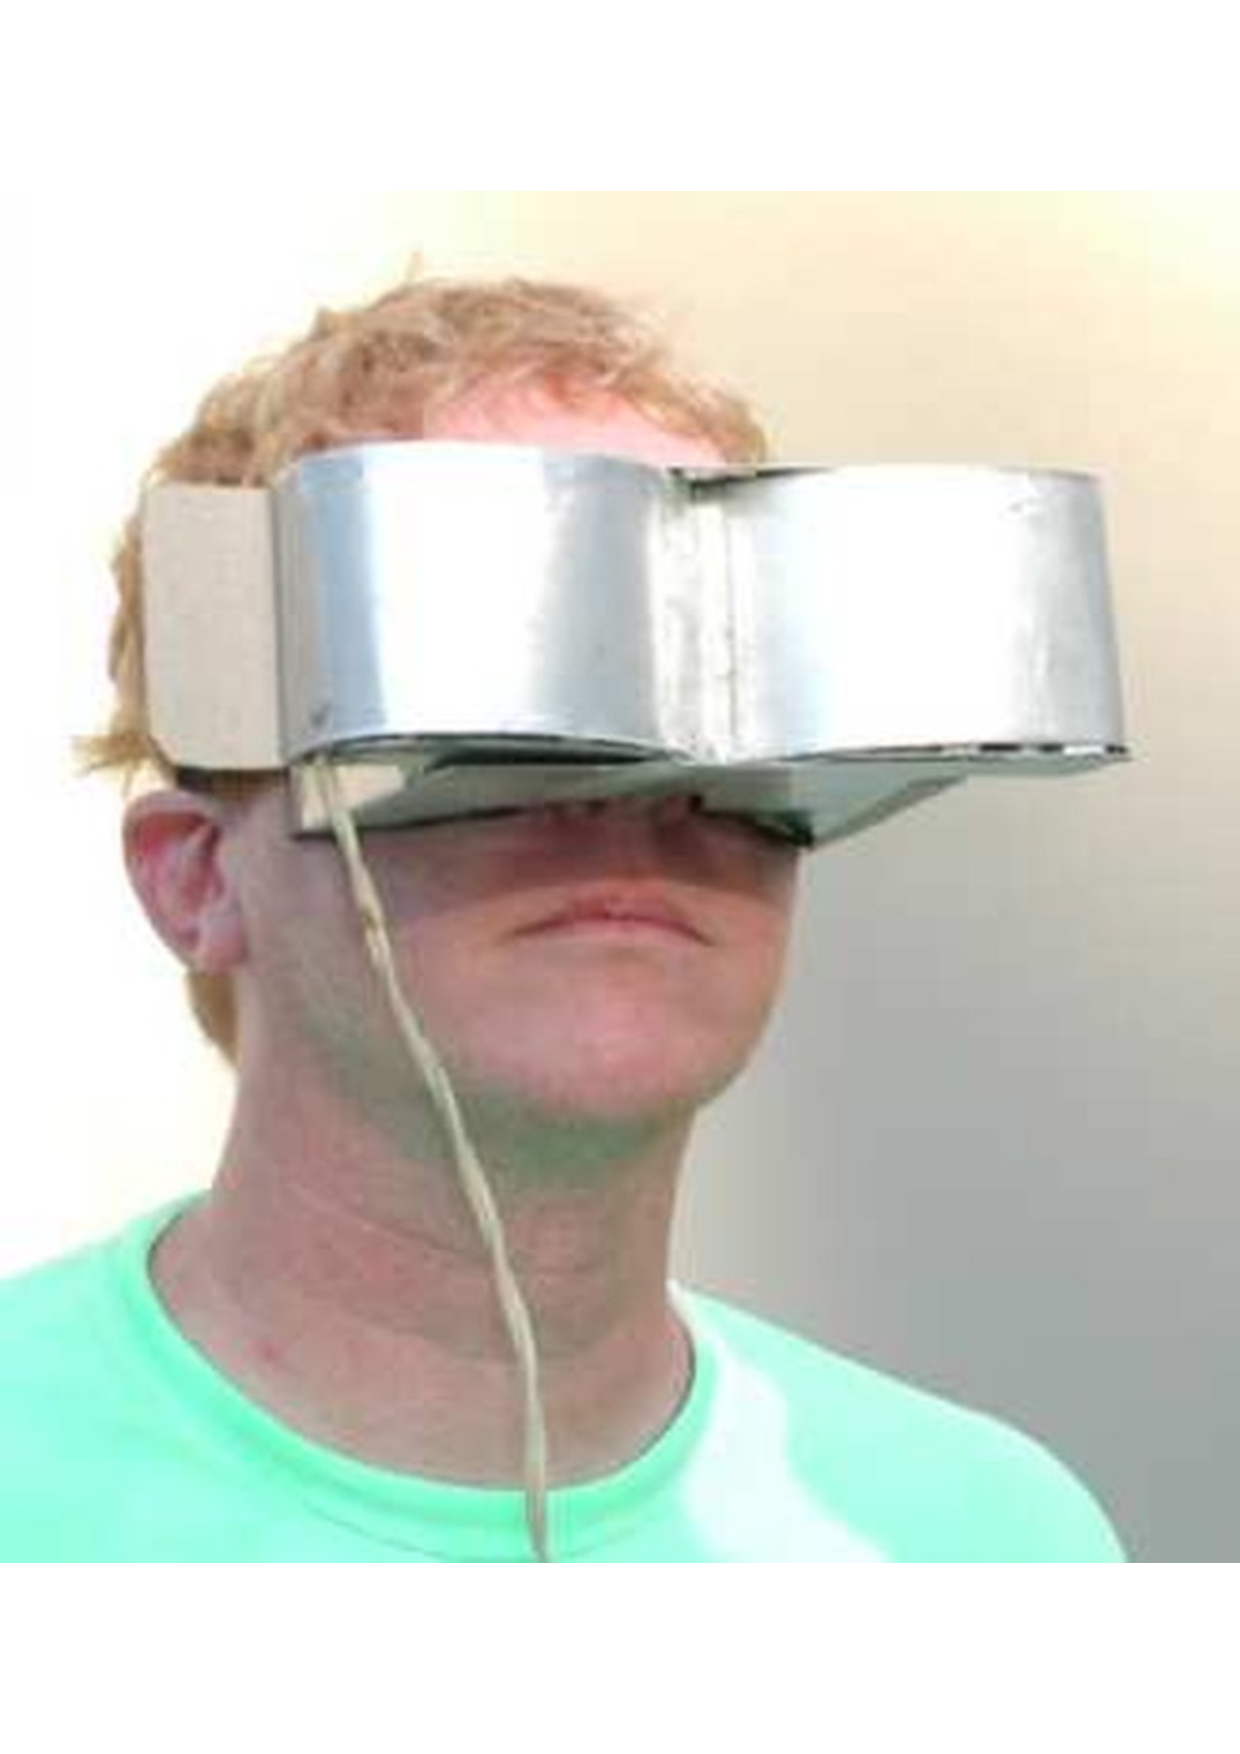
\includegraphics[clip,height=85mm]{Telesphere_Mask.pdf}
\end{center}
 \caption{Telesphere Mask}
 \label{fig:Telesphere_Mask.pdf}
\end{figure}

1970年代にAspen Movie Mapが登場した.図\ref{fig:Aspen_Movie_Map.pdf}のようにヘッドマウントディスプレイでも視界全体を3D映像で覆うことはないが,現在VRコンテンツであるGoogleストリートビューの前身と言われており,アメリカのコロラド州にある街「アスペン」をバーチャルツアーで自由に散策できるというものになっている.
車の天井に装着したカメラでアスペンの街中を撮影し,車が進んでいく様子は動画ではなくパラパラ漫画のように再生される.
スピードは視点を変更したり,一時的に再生を止めるといった操作は「タッチスクリーン」で可能となっている\cite{VRの機材}.

\begin{figure}[h]
\begin{center}
 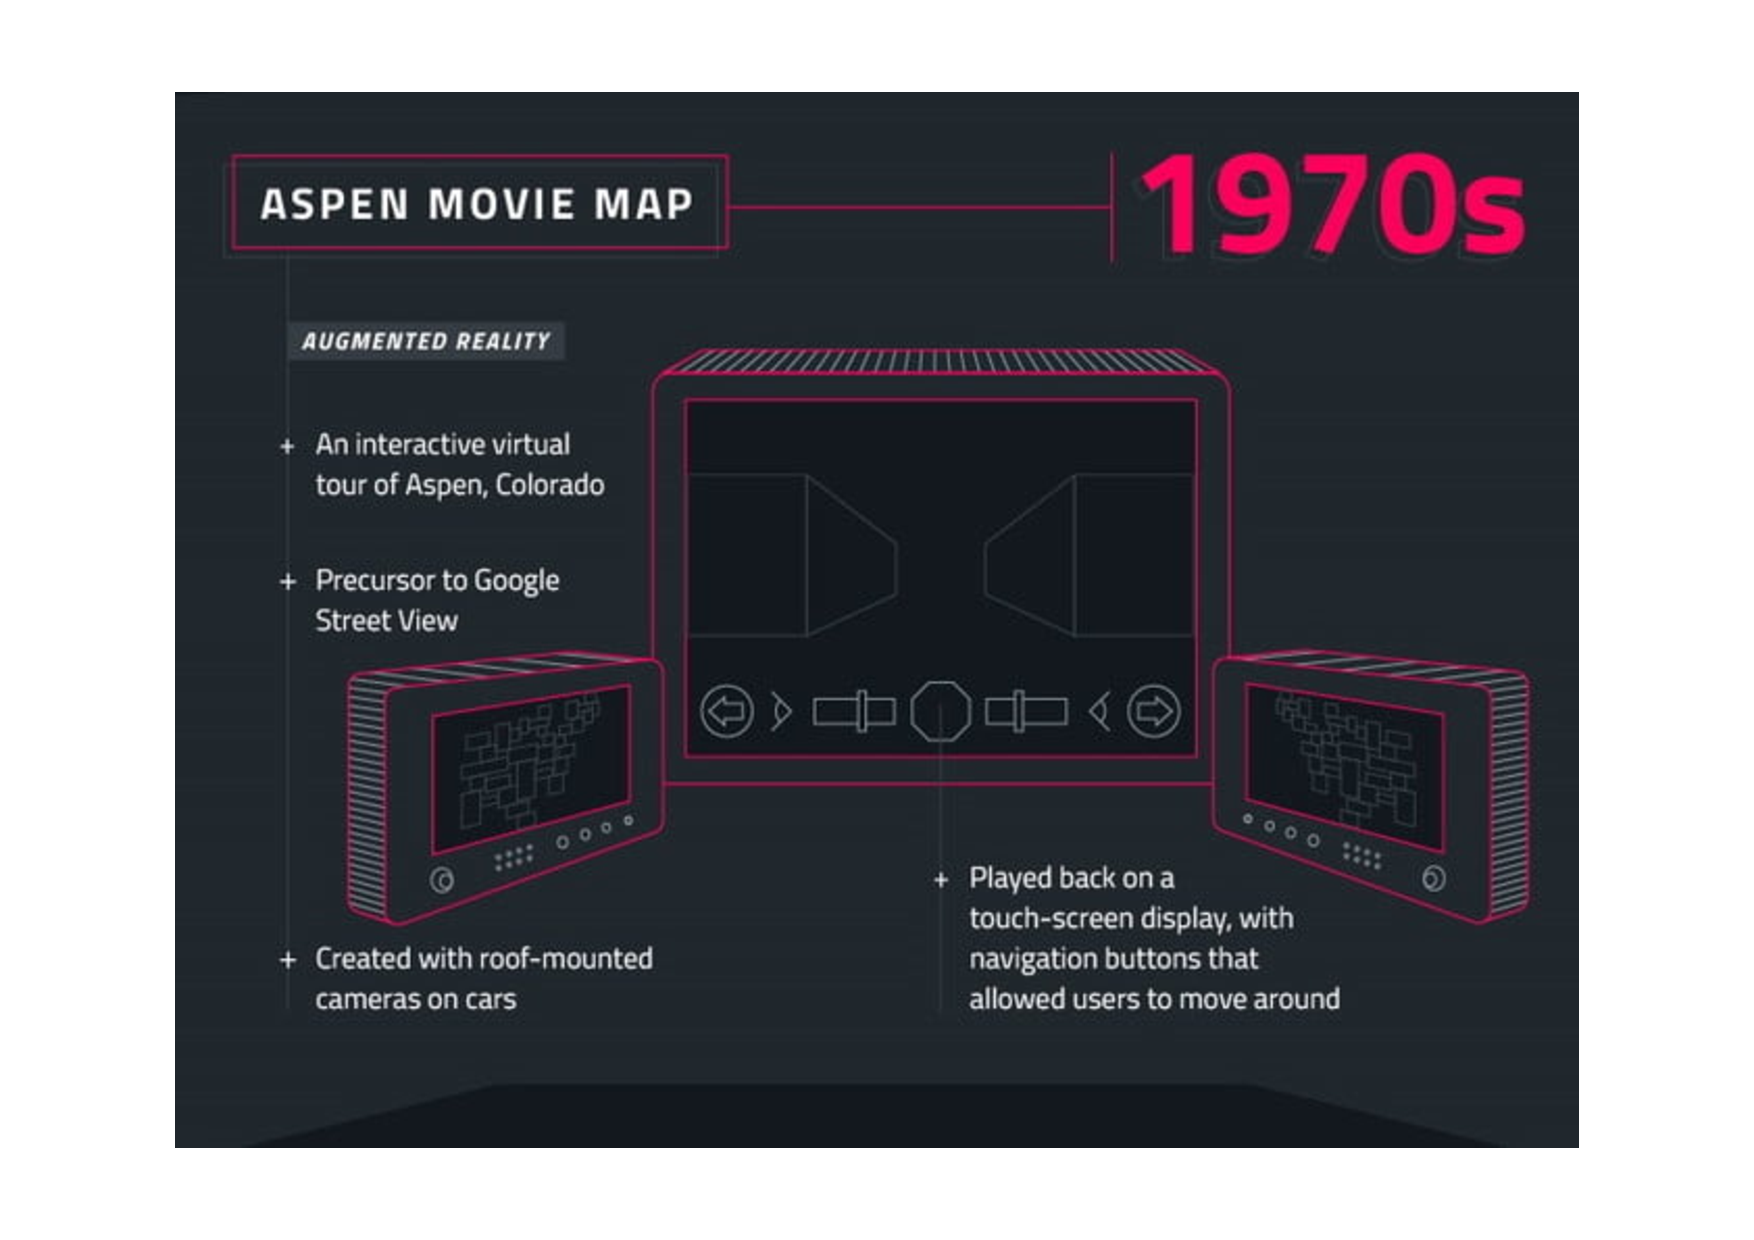
\includegraphics[clip,height=55mm]{Aspen_Movie_Map.pdf}
\end{center}
 \caption{Aspen Movie Map}
 \label{fig:Aspen_Movie_Map.pdf}
\end{figure}

1980年代にThe EyephoneというヘッドマウントディスプレイとThe Data Gloveというグローブ型の入力デバイスが登場した.
この2つは図\ref{fig:The_Eyephone.pdf}のように同時に使うものであり,ヘッドマウントディスプレイの視野角は90°という狭く価格は訳100万円ほどであった\cite{VRの機材}.

\begin{figure}[h]
\begin{center}
 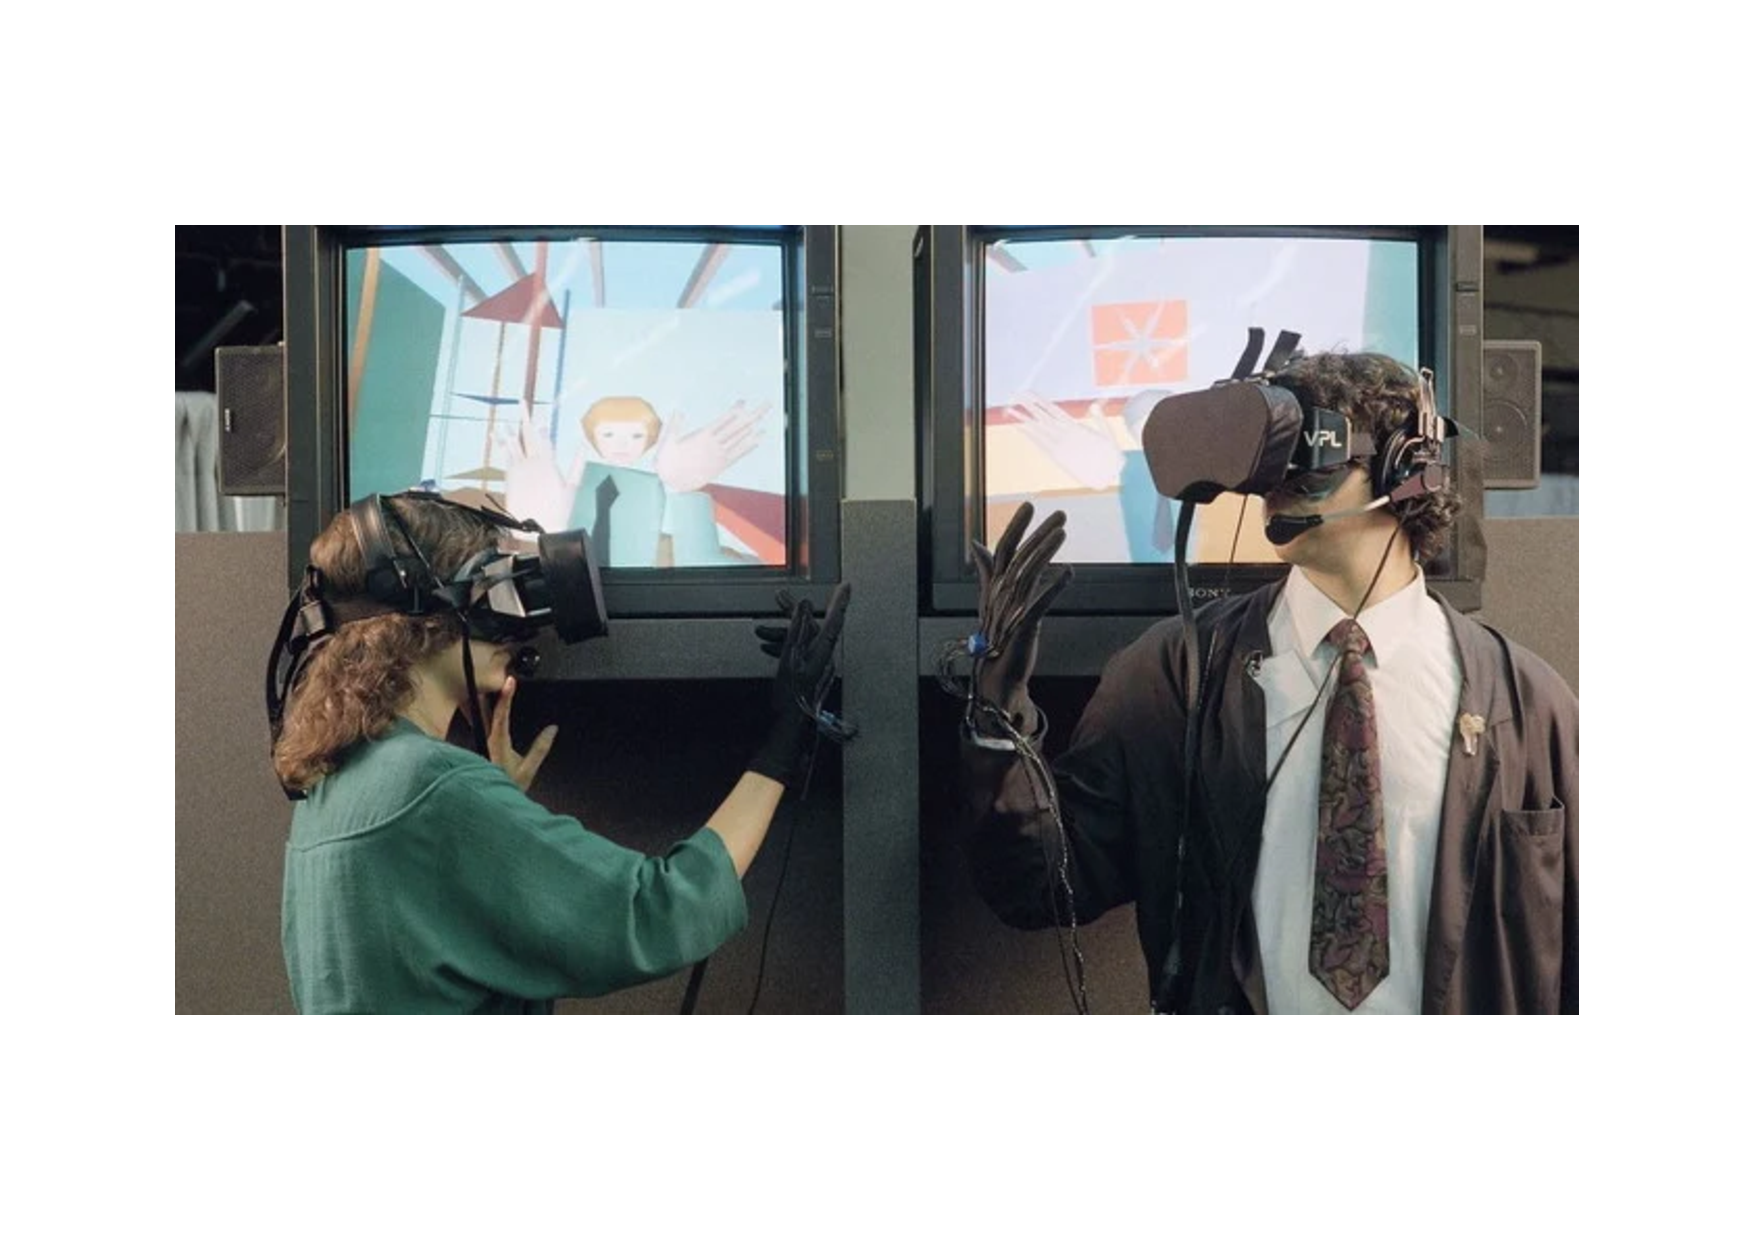
\includegraphics[clip,height=55mm]{The_Eyephone.pdf}
\end{center}
 \caption{The EyeponeとThe Data Glove}
 \label{fig:The_Eyephone.pdf}
\end{figure}

1990年代に任天堂がバーチャル・ボーイを発表した.
このデバイスはスタンドアローン型のデバイスであり,テニスやピンボールなどのコンテンツが遊ぶことができた\cite{VRの機材}.

2010年にモーショントラッキングセンサであるKinectが発売された.Kinectが登場する以前は数千万円もする大掛かりな機材でモーショントラッキングを行っていたが,Kinectの登場により簡単に比較的安価でモーショントラッキングができるようになったため,VR技術が大きく進歩していった\cite{VRの機材}.

2010年以降に図\ref{fig:Google_CardBord.pdf}のようにスマートフォンを利用し安価でVRを利用すことができる段ボール製のデバイスや図\ref{fig:Meta_Quest2.pdf}のようにスタンドアローン型で性能の高いトラッキングシステムが搭載されている機材など様々なものが誕生していった.
\begin{figure}[h]
\begin{center}
 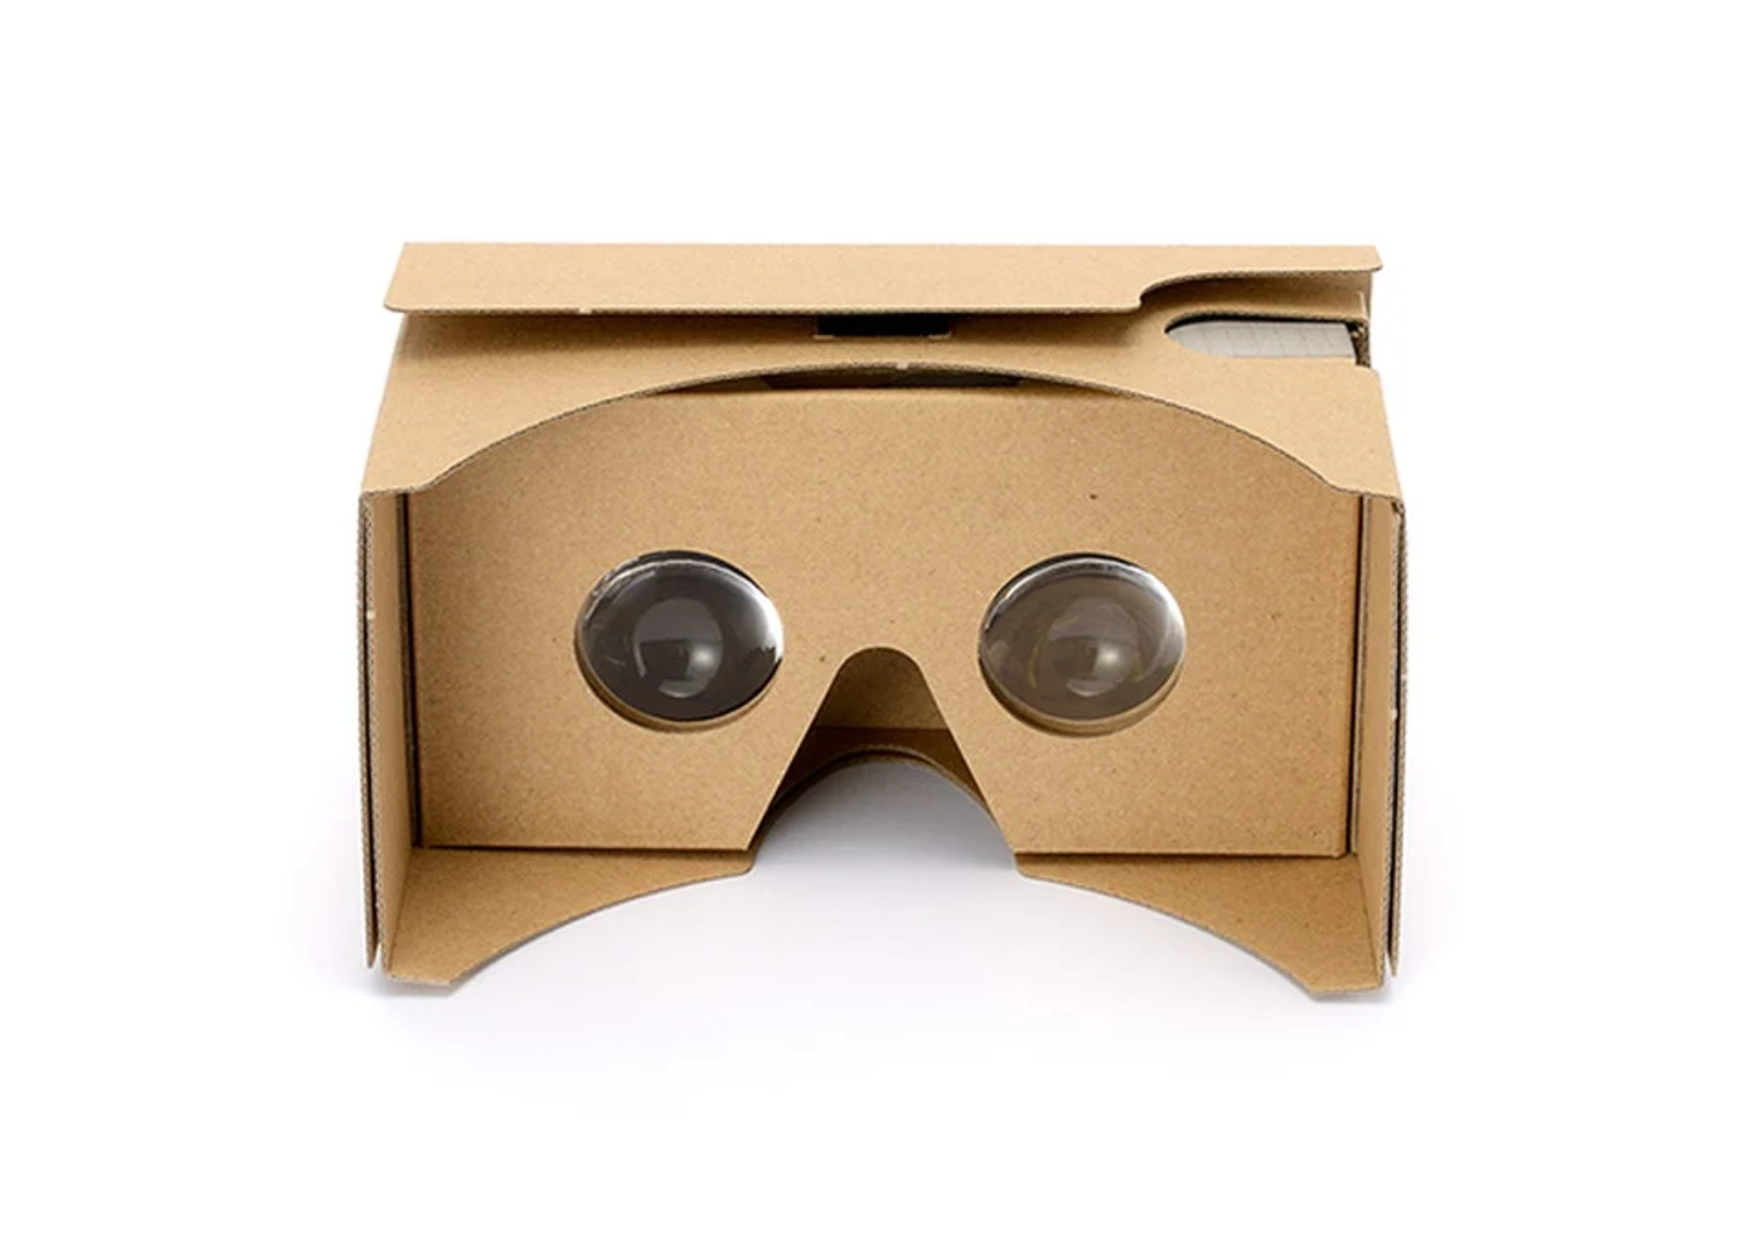
\includegraphics[clip,height=55mm]{Google_CardBord.pdf}
\end{center}
 \caption{Google CardBoard}
 \label{fig:Google_CardBord.pdf}
\end{figure}

\begin{figure}[h]
\begin{center}
 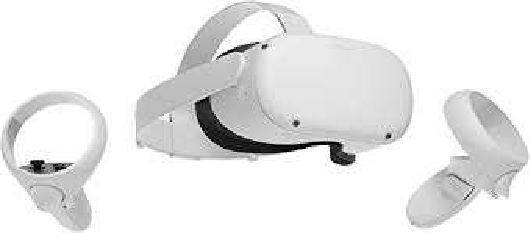
\includegraphics[clip,height=55mm]{Meta_Quest2.pdf}
\end{center}
 \caption{Meta Quest2}
 \label{fig:Meta_Quest2.pdf}
\end{figure}

\subsection{ARの機材}
1968年に登場したThe Sword of DamoclesはARの始まりの機材と言われている.
この機器はコンピュータグラフィックで作られた環境を仮想体験できる装置だが,機材がとても重かったため天井から吊り下げて使う必要があり実用的ではなかった.

AR専用の機器は登場することは少なく,AR技術は主にシステムの進化である.
システムが進化していきそのシステムを様々なヘッドマウントディスプレイやカメラにに搭載していった.

2013年にグラス型のARデバイスが発表され,そこからグラス型ARデバイスが多く登場するようになった.
グラス型のARデバイスは,軽量化がされておりハンズフリーで使用することができることが利点である.
現在のグラス型のARデバイスができることは,動画やメールの閲覧,通話,録音や撮影,健康管理,翻訳,現実にデジタルデータを重ねる,見ている現実の共有ができる\cite{グラス型ARデバイス}.

\subsection{MRの機材}
MR技術専用のデバイスは,グラス型の機材とヘッドマウントディスプレイの2種類がある.

グラス型のMRデバイスは,図\ref{fig:Microsoft_HoloLens.pdf}のようにグラス型のARデバイスと同様の形をしており,透明型の画面で現実世界の上にアプリケーションなどを起動できるデバイスである.

\begin{figure}[h]
\begin{center}
 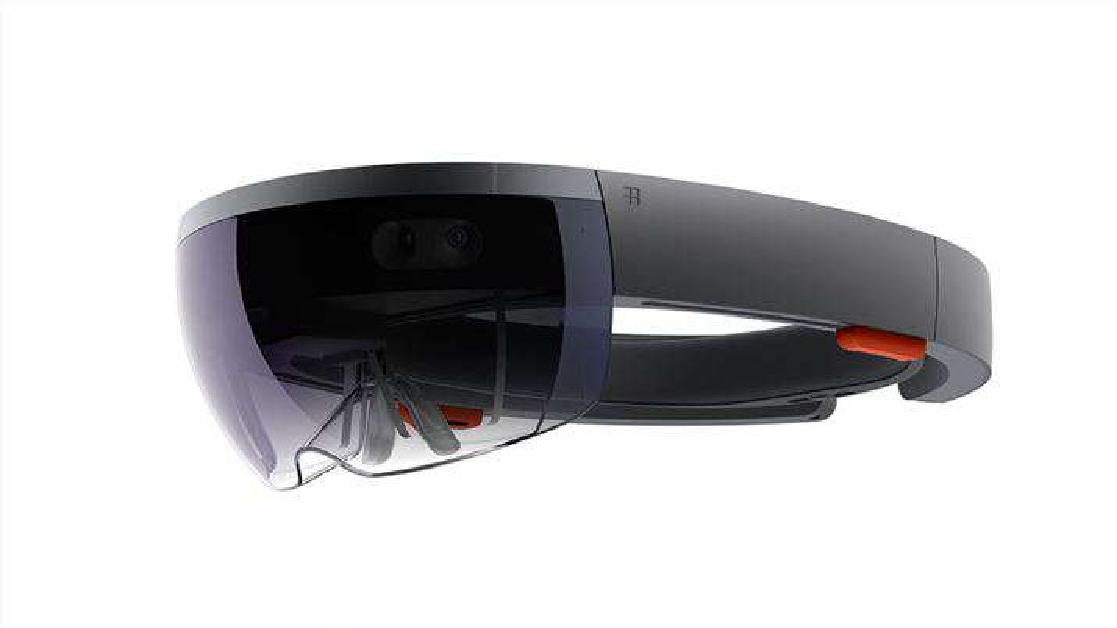
\includegraphics[clip,height=55mm]{Microsoft_HoloLens.pdf}
\end{center}
 \caption{Microsoft HoloLens}
 \label{fig:Microsoft_HoloLens.pdf}
\end{figure}

ヘッドマウントディスプレイは,見た目も機能もVRのヘッドマウントディスプレイと変わらない.
最近では,VRとMRを1つの機器で利用出来るものも登場している.
\clearpage

\section{第1回目のアンケート}
本研究では,Google Formsを利用し千葉工業大学情報科学部情報ネットワーク学科の生徒を対象にアンケートを取った.
アンケートの対象として大学生を選んだ理由としては,大学生は高校生などのほかの学生と違い比較的に多くのお金を持っていて,就職している人たちと比べて自由に使える時間が多いため, xR技術に触れる機会が多いと考えたからである.

\subsection{仮説}
VR技術があまり利用されていない原因としてコンテンツ面に問題があるのではないかと仮説を立てた.
理由は,現在のVR機材の価格は安いものは数百円のものがあり,Nintendo SwitchやPlayStation4などの人気ゲーム機と同じくらいの値段のものが存在するが,あまり利用されていない.
そこにはゲーム機やPCなどの機材との性能の差ではなく,ユーザーが求めているコンテンツがないのではないかと考えたからである.

\subsection{内容}
仮説を元に以下のアンケートを作成した.

アンケートは対象者全員,VRを体験したことがある人,VRを体験したことがない人,VR機器を持っている人,VR機器を持っていない人の5つに分けて質問を作成した.

\subsubsection{対象者全員への質問}
質問の内容は,複数回のアンケートを想定していたため名前で集計し,VR体験をしたことあるかの質問をした.

VR体験をしたことある場合は,VR体験をしたことがない人へのアンケートに飛び,VR体験をしたことがない場合はない人へのアンケートに飛ぶようになっている.

\subsubsection{VR体験をしたことのある人への質問}
質問の内容は,VR機器を所持したことがあるか,VRを体験をして印象に残ったもの,今後体験したいVRコンテンツを質問した.
VR機器を所持したことがあるかの質問はその後VR機器を持っている人アンケートとVR機器を持っていない人へのアンケートのどちらかに分けるための質問である.
VRを体験して印象に残ったものは,どのようなコンテンツがVRを感じれるかの質問である.
今後体験したいVRコンテンツは,VRを知っている中で求められているコンテンツはどのようなものかの質問である.

\subsubsection{VRを体験したことない人への質問}
質問の内容は,体験をしてこなかった理由,どのようなコンテンツを体験してみたいかの質問をした.
体験してこなかった理由という質問は,VRへの印象調査と利用されない理由の調査である.
どのようなコンテンツを体験してみたいかの質問は,VRのことをあまり知らない中で求められているコンテンツの調査である.

\subsubsection{VR機器を所持している人への質問}
質問の内容は,VR機器の購入理由,現在も利用しているか,現在も利用している場合どのようなコンテンツを現在は利用しているのか,利用していない場合利用しなくなった理由,VR機器を他人に勧めたいかを質問した.
VR機器の購入理由の質問は,どのような理由でVR機器を求めたかの質問である.
現在も利用しているかの質問は,利用を継続しているかの調査だけではなく,現在も利用している場合どのようなコンテンツを利用しているかの質問と現在は利用していない場合利用しなくなった理由の質問に分けるための質問でもある.
現在も利用している場合の質問は,どのようなコンテンツが利用され続けられるのかとどのようなコンテンツを求めて利用しているかの調査である.
現在は利用していない場合利用しなくなった理由の質問は,VR機器またはコンテンツの欠点を調査する質問である.
VR機器を他人に勧めたいという質問は,VRを知った上でVR技術は人に勧めたいと思うのかという調査を目的としている.

\subsubsection{VR機器を所持していない人への質問}
質問の内容は,VR機器を購入を考えたことがあるか,VR機器を所持するまでに至らなかった理由,どのようなコンテンツがあるとVR機器を購入するかを質問した.
VR機器の購入を考えたことがあるかの質問は,一般的にVRが欲しいかの調査である.
VR機器を所持するまでに至らなかった理由という質問は,VRが一般的に利用されない理由の調査である.
どのようなコンテンツがあるとVR機器を購入するかの質問は,VRが一般的に使われるようになるにはどのようなコンテンツが求められているのかの調査である.

\subsection{結果}
1回目のアンケートでは,123人に回答してもらった.

\subsubsection{対象者全員への質問}
この質問には,対象者全員への質問のため123人が回答した.

VR体験をしたことがあるかという質問の結果を図\ref{fig:アンケート結果1_1_2.pdf}に示す.
あると答えた人は43人,ないと答えた人は80人だった.
この結果から半数以上の人はVR体験をしたことがないことがわかる.

\begin{figure}[h]
\begin{center}
 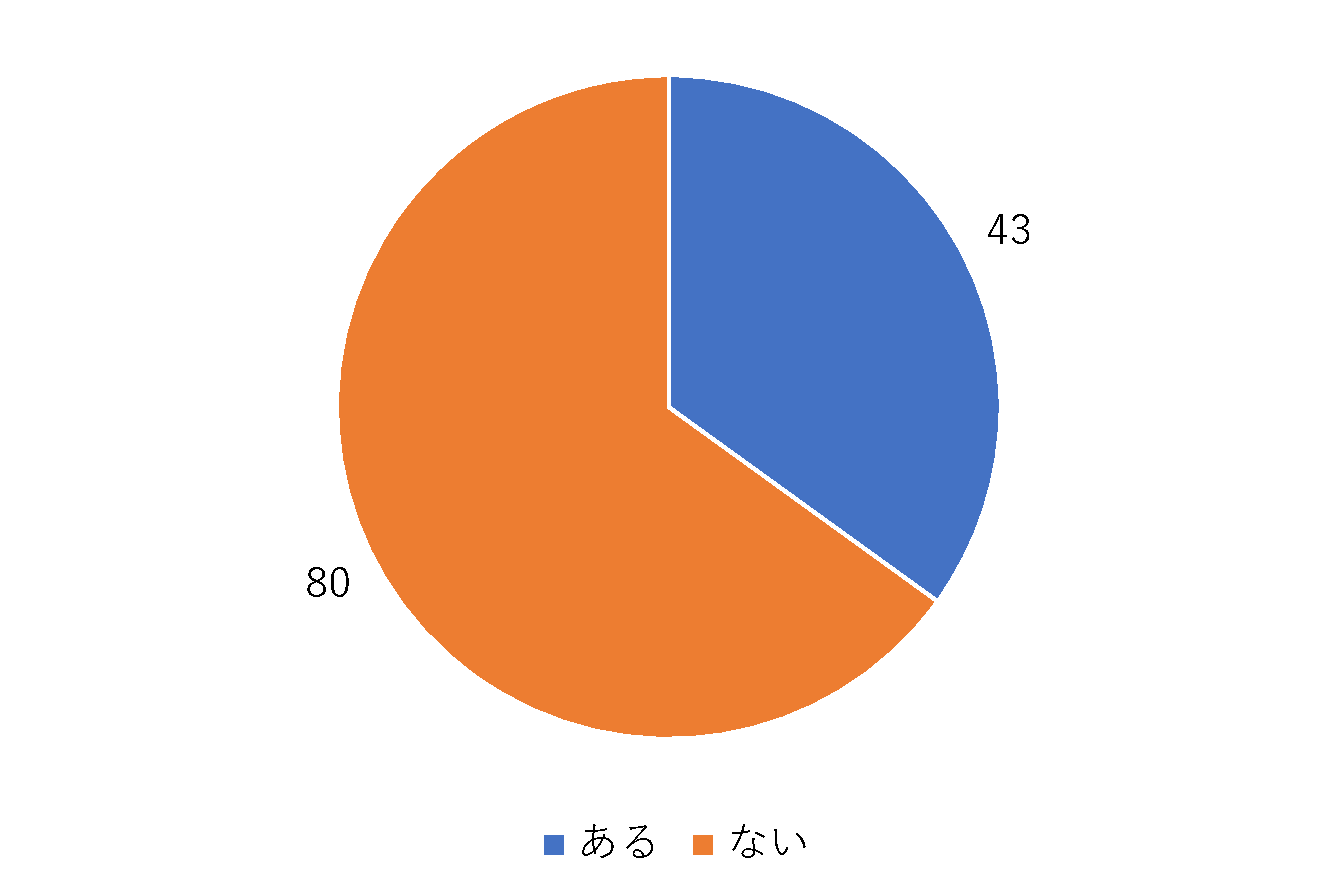
\includegraphics[clip,height=55mm]{アンケート結果1_1_2.pdf}
\end{center}
 \caption{質問1.2 VR体験をしたことがあるか}
 \label{fig:アンケート結果1_1_2.pdf}
\end{figure}

\subsubsection{VR体験をしたことのある人への質問}
この質問は,VR体験をしたことがあると答えた43人が回答した.

VR機器を所持しているかという質問の結果を\ref{fig:アンケート結果1_2_1.pdf}に示す.
43人中15人が所持したことがあると答えている.

\begin{figure}[h]
\begin{center}
 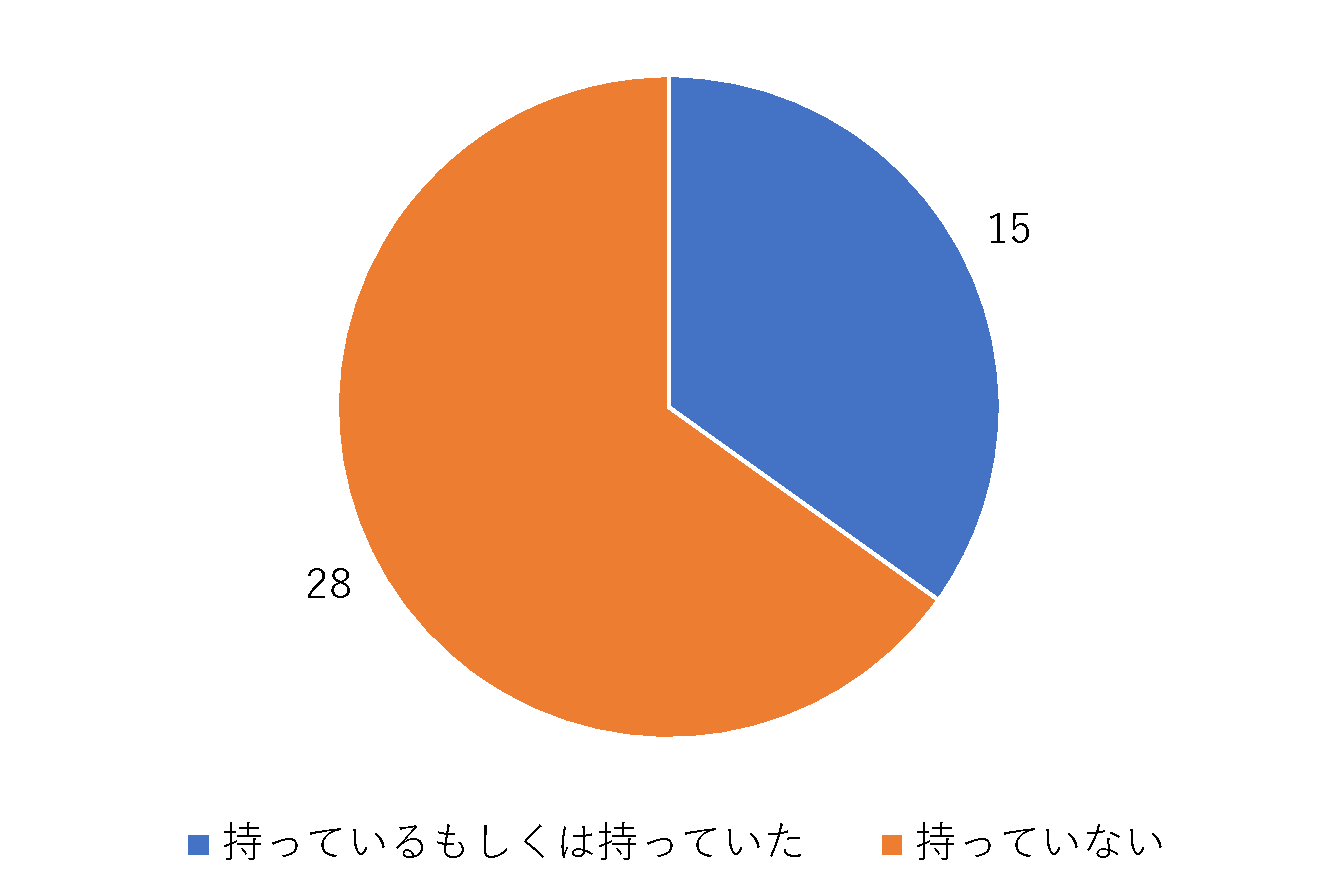
\includegraphics[clip,height=55mm]{アンケート結果1_2_1.pdf}
\end{center}
 \caption{質問2.1 VR機器を所持していますか?}
 \label{fig:アンケート結果1_2_1.pdf}
\end{figure}

印象に残ったVRコンテンツは大きく分けて3種類あった.
ジェットコースターの体験やサメに襲われるなどといった映像を見て体験をするコンテンツ,アクションゲームやVRChatなどといった仮想空間に入り込むコンテンツ,BeatSaberや卓球をするなどといった体を動かすコンテンツの3種類に分かれていた.

今後体験してみたいコンテンツは,現実世界では行うことが困難なことやライブといった仮想世界なら体験が容易になるコンテンツや,VRアバターを使ったコミュニケーションコンテンツ,仮想世界に入り込むゲームのように非現実的なコンテンツが求められていた.

\subsubsection{VRを体験したことない人への質問}
この質問にはVR体験をしたことがないと答えた80人が回答した.

VR体験をしてこなかった理由は何かという質問の結果を図\ref{fig:アンケート結果1_3_1.pdf}に示す.
複数回答が可能な質問であり最も多かった回答は機会がなかったことだ.
次にVRを体験できる施設を知らないという回答が多かった.
VR技術に興味が無かったりVRを体験すると体調が悪くなると考える人いた.

\begin{figure}[h]
\begin{center}
 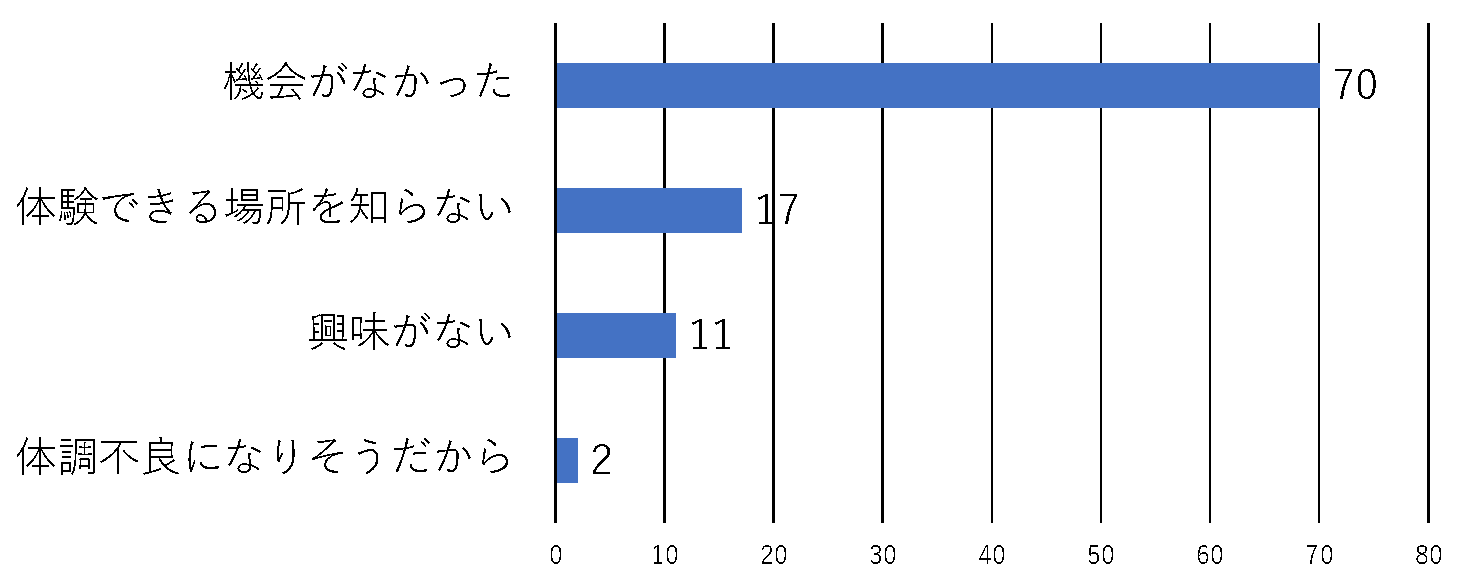
\includegraphics[clip,height=55mm]{アンケート結果1_3_1.pdf}
\end{center}
 \caption{質問3.1 VR体験をしてこなっかった理由はなんですか?}
 \label{fig:アンケート結果1_3_1.pdf}
\end{figure}

どのようなVRを体験したいかという質問は,VRを体験した人よりも種類が多く仮想世界に入ることやホラーなどといった非現実的な体験をするコンテンツ,ライブやジェットコースターなどの体験型コンテンツ,VRChatのようなコミュニケーションコンテンツ,野球などのスポーツを体験するコンテンツ,海外に旅行したような体験ができるコンテンツなどがあった.

\subsubsection{VR機器を所持している人への質問}
この質問はVR機器を持っているまたは持っていたことがあると答えた15人が回答した.

VR機器を所持した理由について聞いたところ,VR技術に興味があって購入した人が12人,家族が購入したのが3人という結果だった.
現在もVR機器を利用しているかという質問の結果を図\ref{fig:アンケート結果1_4_2.pdf}に示す.
3人は利用していて12人は利用しなくなった.
また現在も利用している人の共通点として購入理由の時に利用したいコンテンツがあると答えている.
\begin{figure}[h]
\begin{center}
 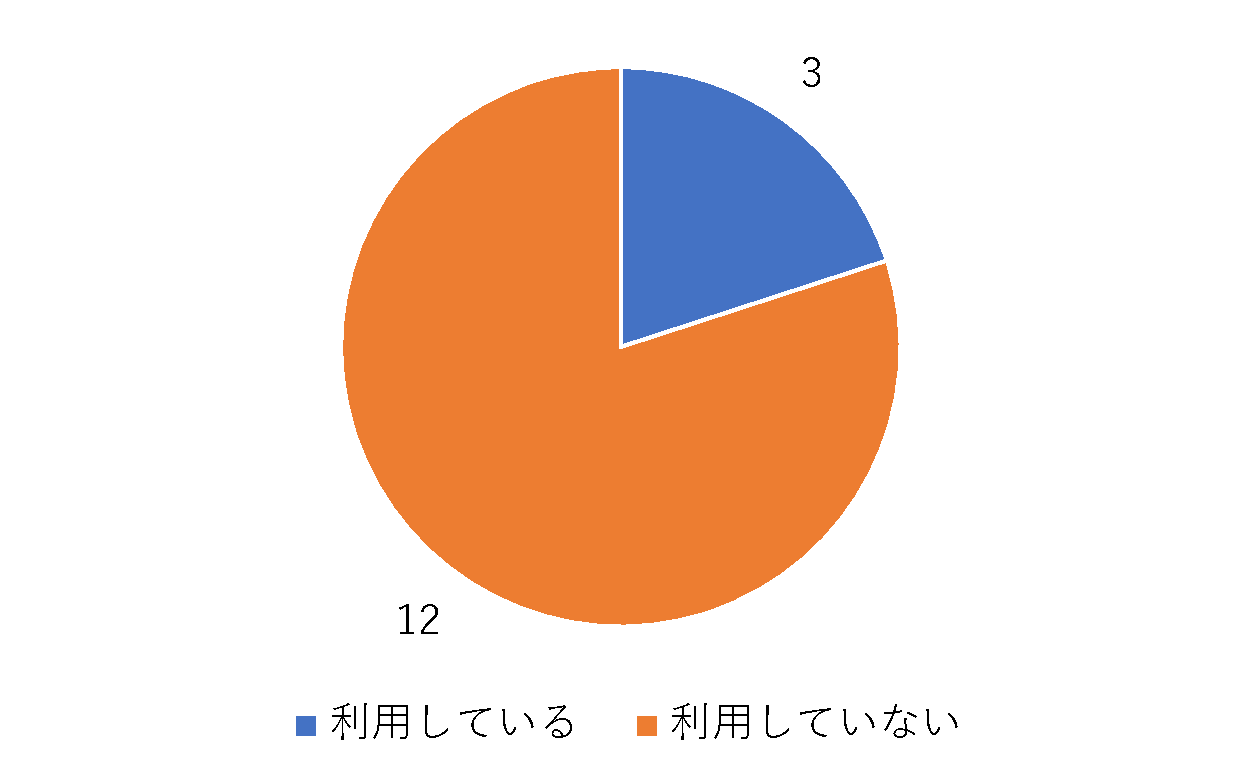
\includegraphics[clip,height=55mm]{アンケート結果1_4_2.pdf}
\end{center}
 \caption{質問4.2 現在も利用していますか?}
 \label{fig:アンケート結果1_4_2.pdf}
\end{figure}
現在も利用している人は,現在はコミュニケーションコンテンツや動画の視聴をするために利用していると答えた.
利用をやめてしまった人は,機材が重たいことや性能が低いといった機材面の問題,やりたいコンテンツが無くなったやVRに興味がなくなったといった理由で利用をやめたと答えた.

VR機器の購入を勧めたいと思うかという質問の結果をず\ref{fig:アンケート結果1_4_5.pdf}に示す.
勧めたいと思う人が10人勧めたくないと思う人が5人いた.
\begin{figure}[h]
\begin{center}
 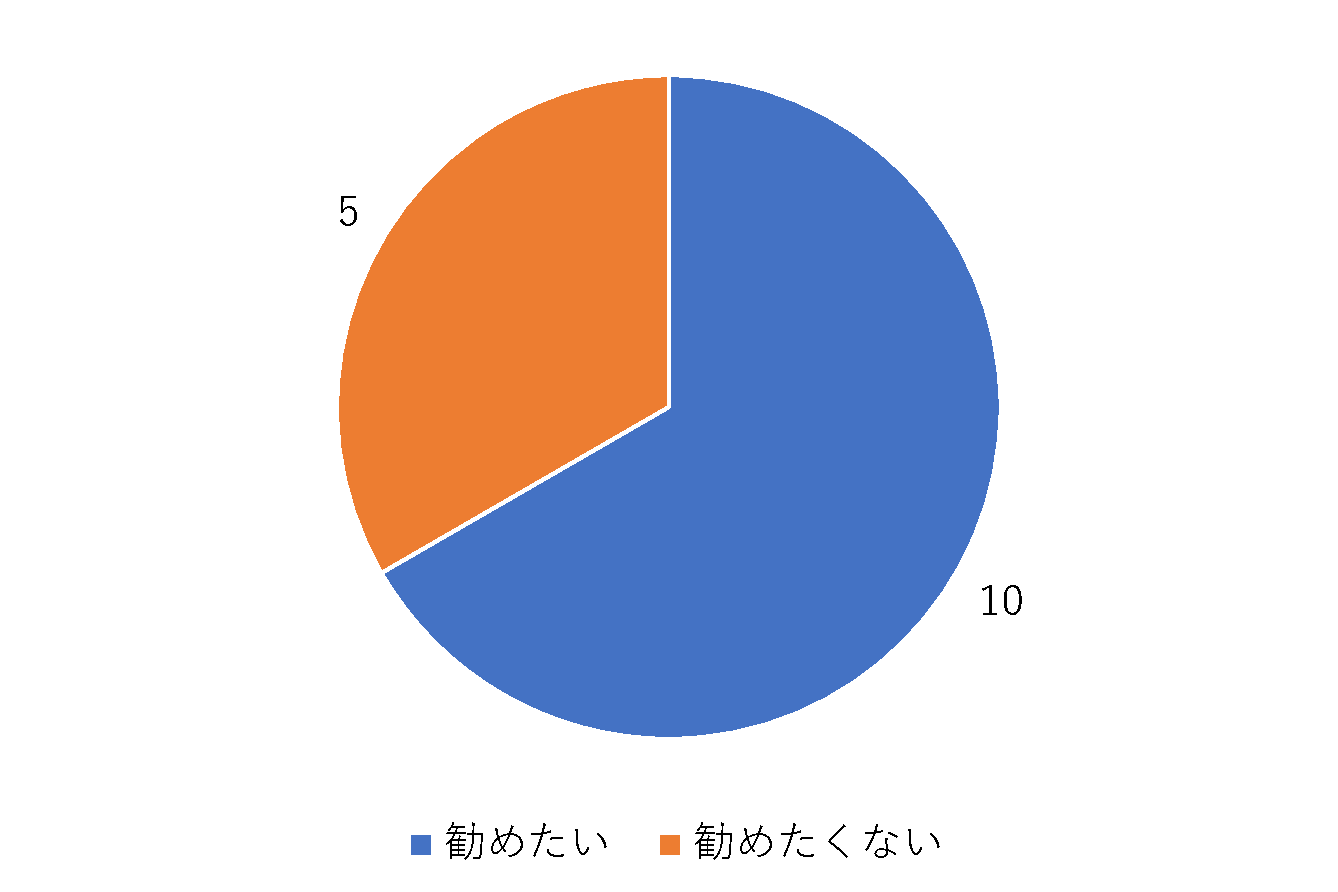
\includegraphics[clip,height=55mm]{アンケート結果1_4_5.pdf}
\end{center}
 \caption{質問4.5 VR機器の購入を人に勧めたいと思いますか?}
 \label{fig:アンケート結果1_4_5.pdf}
\end{figure}

\subsubsection{VR機器を所持していない人への質問}
VRを体験したことがないと答えた人とVR機器を持っていないと答えた人の合計108人が回答した.

VR機器の購入を考えたことがあるかという質問は,考えたことがあると回答した人が30人考えたことがないと回答した人が78人という結果だった.

\begin{figure}[h]
\begin{center}
 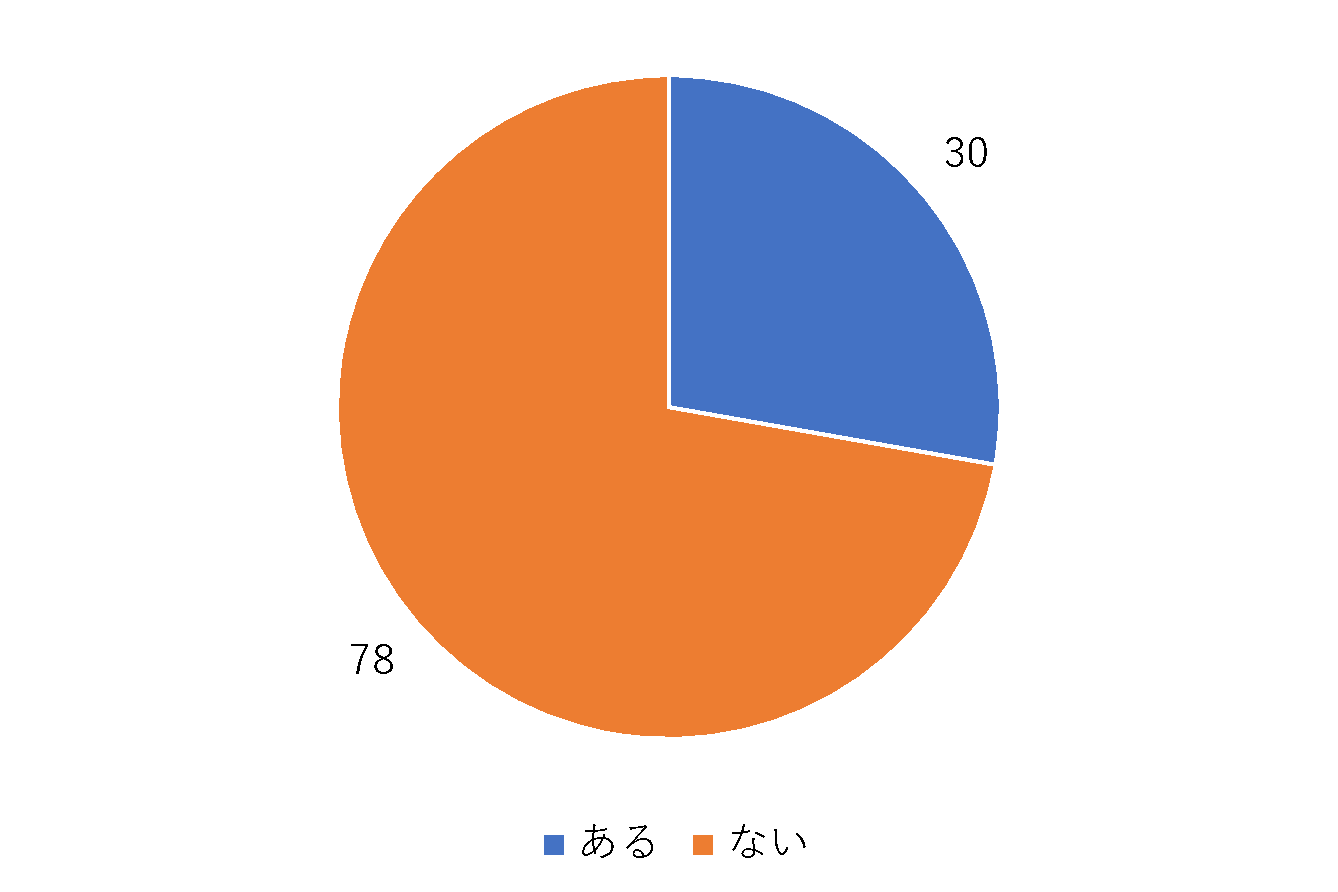
\includegraphics[clip,height=55mm]{アンケート結果1_5_1.pdf}
\end{center}
 \caption{質問5.1 VR機器を購入しようと考えたことはありますか?}
 \label{fig:アンケート結果1_5_1.pdf}
\end{figure}

所持するまでに至らなかった理由として最も多かった意見は機材が高価だという意見である.
利用したい場所がない,VRに興味がない,利用したいコンテンツがないという意見もあった.
少数意見ではあるがVR技術を利用すると体調不良になったり買う優先度が低い,手軽ではないという意見もあった.

どのようなコンテンツがあるとVR機器を購入するかという質問で多かった意見は,完全にゲームの世界に入り込むコンテンツや有名タイトルのゲームのVR化,機材が安価になれば買うという意見である.
他にも映画や日本では体験できないことなどといった現実では体験することが難しいコンテンツ,全身を動かすコンテンツ,より現実に近いコンテンツなども回答されていた.

\subsubsection{結果から生まれた疑問}
1回目のアンケートから新たに疑問が3個生まれた.
1つ目は,VRを体験したことが少ないという点からそもそもVRを体験していないためVRのことがよくわからないから利用しないのではないか,
2つ目は,コンテンツの問題より機材面に問題があるのではないか,
3つ目は,VRコンテンツには知名度のあるものが求められているのではないかという3個の疑問が生まれた.

\clearpage

\section{第2回目のアンケート}
1回目のアンケートで出た新たな疑問を元に2回目のアンケートを行った.
2回目のアンケートも1回目のアンケート同様Google Formsを利用し千葉工業大学情報科学部情報ネットワーク学科の生徒を対象にアンケートを取った.

\subsection{仮説}
1回目のアンケートをもとに立てた新たな仮説を立てた.
VR体験をしていないからVRのことがよくわからない,機材面に問題がある,知名度のあるコンテンツが求められているというて問題点から知名度が高いVRコンテンツがあり機材が安価になるまたは安価で体験できる施設が増えて気軽に体験できるようになると利用者が増えるのではないかというに新たな仮説である.

\subsection{内容}
仮説を元に以下のアンケート作成した.

アンケート対象者全員,金額によっては購入しても良い人,安くても購入したいと考えない人,VRコンテンツについての4つに分けて質問を作成した.

今回は,VR技術とVR機器の詳細をアンケートに載せ,それを読んだ上で回答してもらった.

VRについては,首を回すと画面が実際に首を回したように動く,コントローラーをもった手を動かすとVR空間内にある手が動くなどの利用者に合わせてVR空間のアバターも動く.安い機材ではVRアバターを動かすことができないが,高い機材になっていくにつれ動かせる幅や精度も上がっていくと記述した.

VR機材については500円で販売されている機材,7000円で販売されている機材,3万円で販売されている機材,6万円で販売されている機材,22万円で販売されている機材に分けて詳細を説明した.
早見表で必要機材,コントローラの数,フレームレート,アイトラッキング機能の有無,価格帯を示し,値段別の機器の特徴を記述した.
またジャイロ機能を使用した時に顔の振り向きに対してVR画面の切り替わりの差についても記述しこれらを読んだ上で回答してもらった.

\subsubsection{対象者全員への質問}
質問内容は,前回のアンケートの回答と比較するために名前で集計し,値段が何円までであれば友人に購入を勧めるか,VR体験ができる施設がありいきたいと思うかを質問した.

値段が何円までであれば友人に購入を勧めるかの質問は,機材が高価だという印象が多かったため値段別の性能でどこまでならVR機材にお金を出せるかの質問である.
自分が買うのではなく友人に勧めるという質問にした理由として,自分が買う場合現在の自分の経済状況に左右されてしまうが,友人が買う場合経済状況よりもコストパフォーマンスを重視すると考えたからである.

VR体験ができる施設があり行きたいと思ったかという質問は,1回目のアンケートでVR体験をしたことがない人が多かったためVR技術自体にあまり興味がないのではと考え,VR技術に対して興味があるかの調査である.

\subsubsection{金額によっては購入をお勧めすると考えた人への質問}
質問内容は,VR機器の購入意欲とその理由,詳細を読んでどの機材を友人にお勧めしたいかとその理由を質問した.
VR機器の購入意欲とその理由の質問は,金額によっては購入をお勧めすると考えた人はどのくらいVRに対して興味があるかの調査である.
詳細を読んでどの機材を友人にお勧めしたいかとその理由を質問した理由としては,どの価格帯の性能がちょうどいい性能をそているかの調査である.


\subsubsection{安くても購入したいと考えない人への質問}
質問の内容は,VR機器を購入しない理由,VR機器は高価だと思うか,VR機器がどのくらいの値段だと購入しようと感じるか,購入しようと考えた価格で欲しい機能は何か,VR機器に対する印象は何か,VR機器を友人に勧める場合お勧め度はどのくらいかとその理由を質問した.
VR機器を購入しない理由の質問は,現在のVR技術の欠点を具体的に調査するための質問である.
VR機器は高価だと思うかの質問は,4段階評価で質問することでどのくらい高価だと感じるかの調査である.
VR機器がどのくらいの値段だと購入しようと感じるかの質問は,VR機器に求められている値段はどのくらいかの調査である.
購入しようと考えた価格で欲しい機能は何かの質問は,どの価格でどのような機能が欲しいかの調査である.
VR機器に対する印象は何かという質問は,購入をしたいと考えない人の現在のVRに対する印象の調査である.
VR機器を友人に勧める場合お勧め度はどのくらいかとその理由という質問は,VRがどのくらい期待されているかの調査である.

\subsubsection{VRコンテンツに関する質問}
質問の内容は,4種類のコンテンツを紹介し,それぞれの購入意欲と最も関心のあるコンテンツを質問した.
またVR機材専用のタイトルと別のゲーム機器で有名なタイトルのコンテンツでの比較とアクションゲームとホラーゲームの2ジャンルに分けてどのようなコンテンツが求められるのかを調査した.
1つ目のコンテンツは,Zenith: The Last City というVR空間で剣と魔法を使って冒険していく本格MMORPGゲームである.
このコンテンツは,アクション要素とMMO RPGのためコミュニケーション要素のあるコンテンツであり,VRオリジナルのコンテンツである.
2つ目のコンテンツは,アフェクテッド 恐怖の館という体験型ホラーゲームである.
内容は,お化け屋敷の中を探索するというものである.
多くのホラーシーンと分岐ルートによって長く遊べるVRオリジナルコンテンツである.
3つ目のコンテンツは,バイオハザード4VRという有名タイトルのバイオハザードシリーズのVRコンテンツである.
このコンテンツはアクション要素が多くホラー要素もある作品である.
4つ目のコンテンツは,Among Us VRというスマートフォンでプレイができる宇宙船を舞台にした人狼ゲームである.
このコンテンツは,一時期さまざまな動画サイトで取り上げられ多くの人にダウンロードされた有名タイトルのVRコンテンツである.
提示された任務をこなしながらチーム内にいる裏切るものを探すゲームであるためアクション要素とコミュニケーション要素のあるコンテンツである.

\subsection{結果}
2回目のアンケートには,69人に回答してもらった.

\subsubsection{対象者全員への質問}
この質問には,対象者全員への質問のため69人が回答した.

あなたは値段が何円までであれば友人にVR機器の購入をお勧めしようと思うかという質問の結果は図\ref{fig:アンケート2_1_2.pdf}に示す.
最も多かった回答は10000円であった.
次に多かった価格帯として50000円が次に多かった.
最も少なかったの10万円である.

\begin{figure}[h]
\begin{center}
 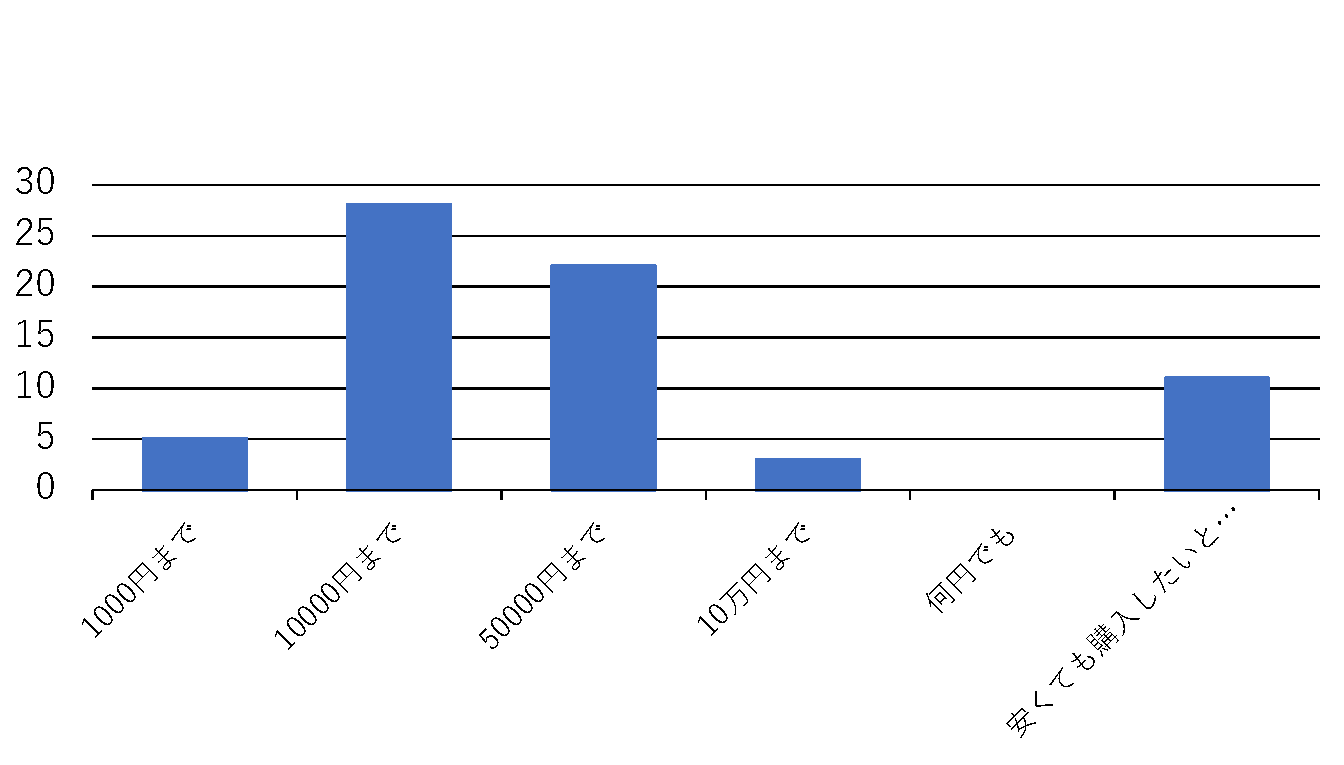
\includegraphics[clip,height=55mm]{
 アンケート2_1_2.pdf}
\end{center}
 \caption{質問1.2 あなたは値段が何円までであれば友人にVR機器の購入をお勧めしようと思いますか?}
 \label{fig:アンケート2_1_2.pdf}
\end{figure}

VR体験ができる施設があり行きたいと思うかという質問の結果は図\ref{fig:アンケート2_1_3.pdf}に示す.
69人中49人が行きたいと答えた.

\begin{figure}[h]
\begin{center}
 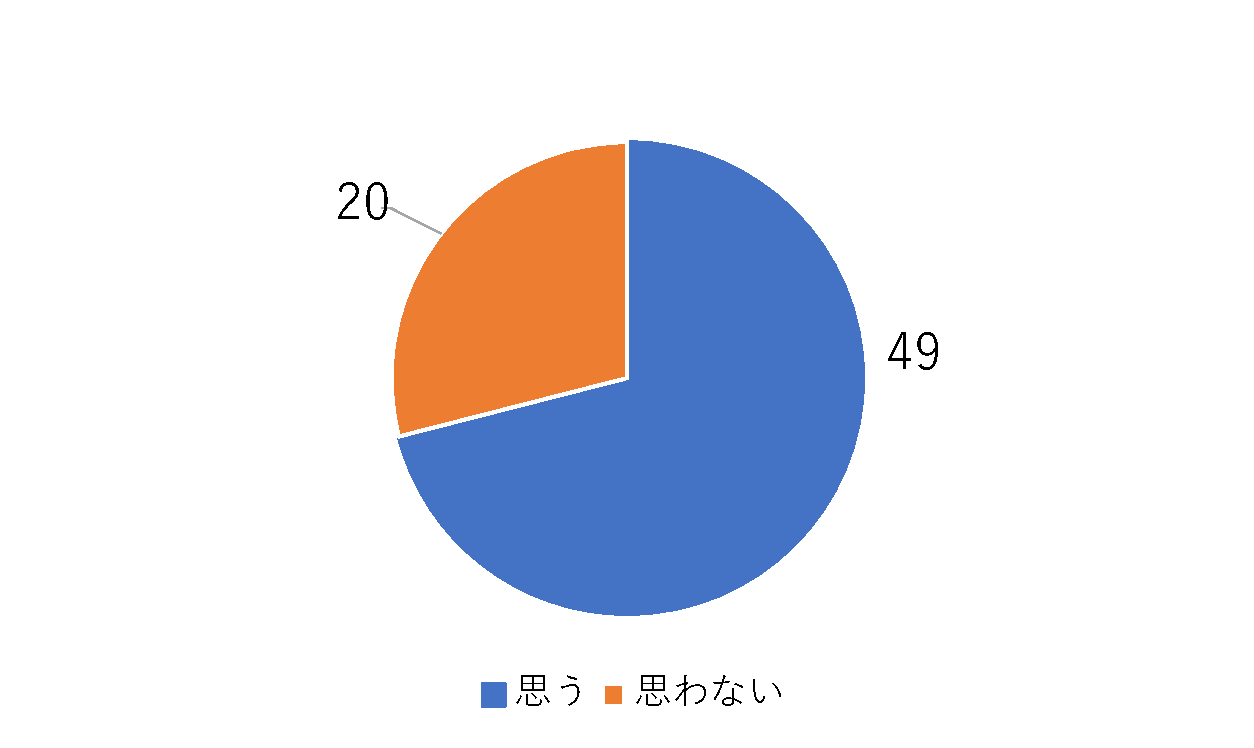
\includegraphics[clip,height=70mm]{
 アンケート2_1_3.pdf}
\end{center}
 \caption{質問1.3 VR技術を体験できる施設が東京にあります。
そこでは1000円で1つのアクティビティができ、アクションや絶叫系アトラクション、ホラーを体験できます。
その施設に行きたいと思いますか?}
 \label{fig:アンケート2_1_3.pdf}
\end{figure}

\subsubsection{金額によっては購入をお勧めすると考えた人への質問}
この質問には,あなたは値段が何円までであれば友人にVR機器の購入をお勧めしようと思うかという質問に安くても購入したいとは思わないという回答をしていない58人に回答してもらった.

購入意欲はどのくらいあるかという質問の結果は図\ref{fig:アンケート2_2_1.pdf}に示す.
最も多かったのは下から2番目くらいで,その次は上から2番目だった.
下から2番目を選んだ人の意見として多いものは,利用してみたいが高価という意見だった.
また購入意欲が高い人の意見は,具体的にやりたいコンテンツがあったり体験してほしいという意見が多かった.

\begin{figure}[h]
\begin{center}
 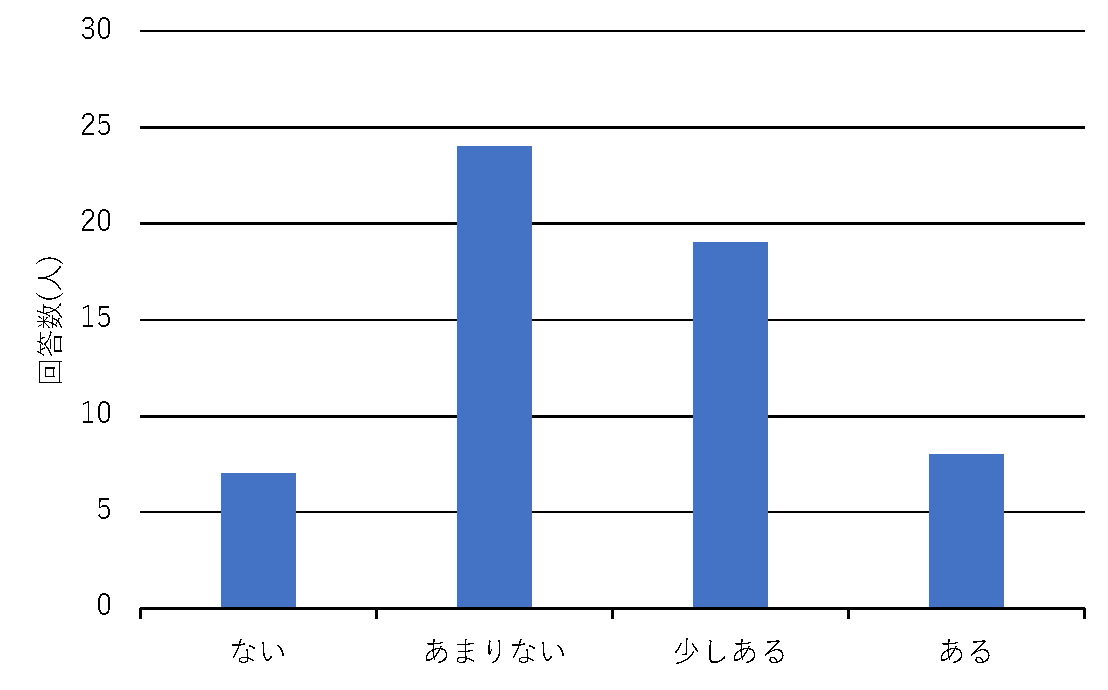
\includegraphics[clip,height=55mm]{
 アンケート2_2_1.pdf}
\end{center}
 \caption{質問2.1 あなたはVR機器への購入意欲はどのくらいありますか?}
 \label{fig:アンケート2_2_1.pdf}
\end{figure}

【値段別VR機器の詳細】の中で購入を勧めることになったらどれが良いという質問の結果は図\ref{fig:アンケート2_2_3.pdf}に示す.
最も多かったのは6万円の機材で23人である.
その次に多かったのは,3万円の機材で11人であった.

その理由としては,性能面が良いからという意見が多かった.
またPCに接続できるという点から汎用性が高いからという意見も多くあった.
お勧めしたいのがないと答えた人は,性能と価格が合わないからという意見だった.

\begin{figure}[h]
\begin{center}
 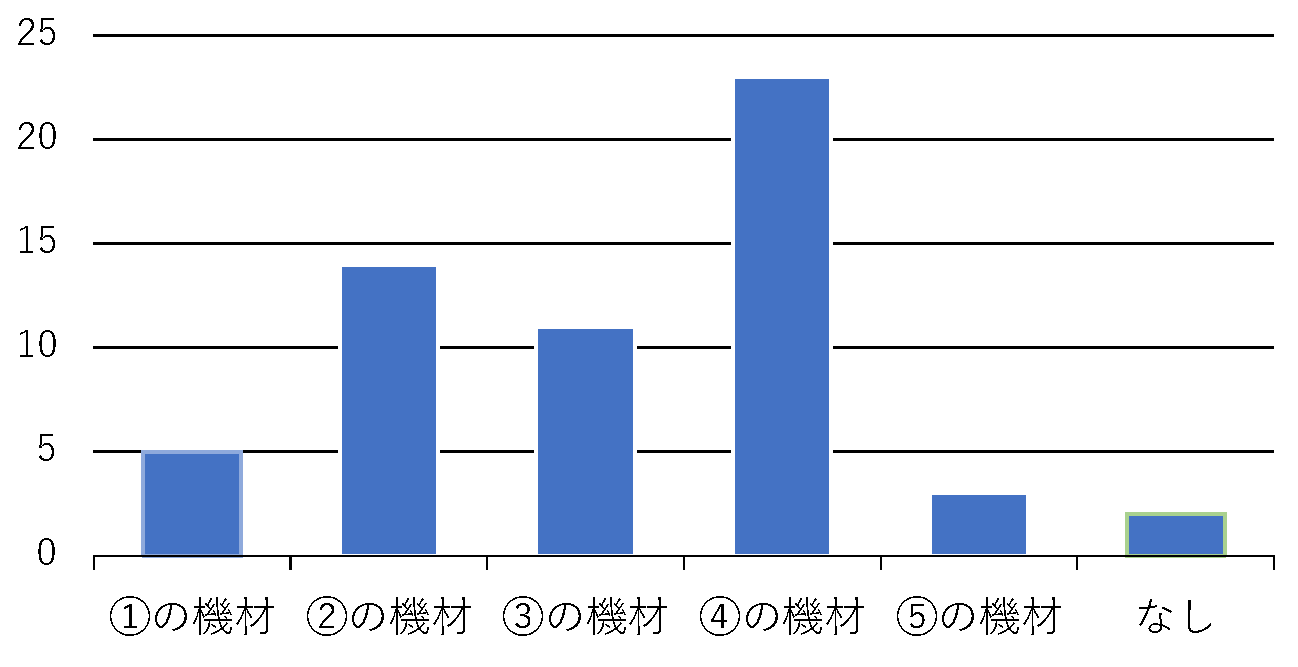
\includegraphics[clip,height=55mm]{
 アンケート2_2_3.pdf}
\end{center}
 \caption{質問2.3 【値段別VR機器の詳細】の中で購入を勧めることになったらどれが良いと考えますか?}
 \label{fig:アンケート2_2_3.pdf}
\end{figure}

\subsubsection{安くても購入したいと考えない人への質問}
この質問には,あなたは値段が何円までであれば友人にVR機器の購入をお勧めしようと思うかという質問に安くても購入したいとは思わないという回答をした11人に回答してもらった.

VR機器を購入しないと考える理由は何かという質問の結果は図\ref{fig:アンケート2_3_1.pdf}に示す.
最も多かったのは興味がないという意見だった.

\begin{figure}[h]
\begin{center}
 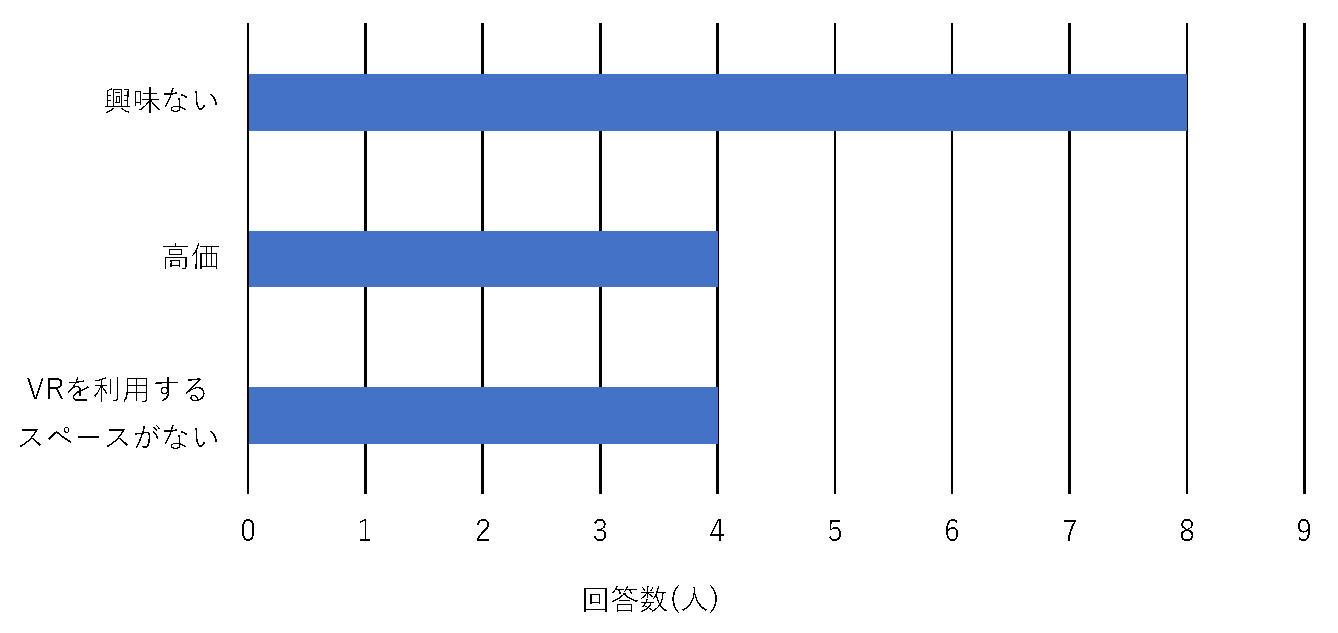
\includegraphics[clip,height=55mm]{
 アンケート2_3_1.pdf}
\end{center}
 \caption{質問3.1 VR機器を購入しないと考える理由は何ですか?}
 \label{fig:アンケート2_3_1.pdf}
\end{figure}

VR機器が高価だと思うかという質問の結果は図\ref{fig:アンケート2_3_2.pdf}に示す.
全員が高価という意見だった.

\begin{figure}[h]
\begin{center}
 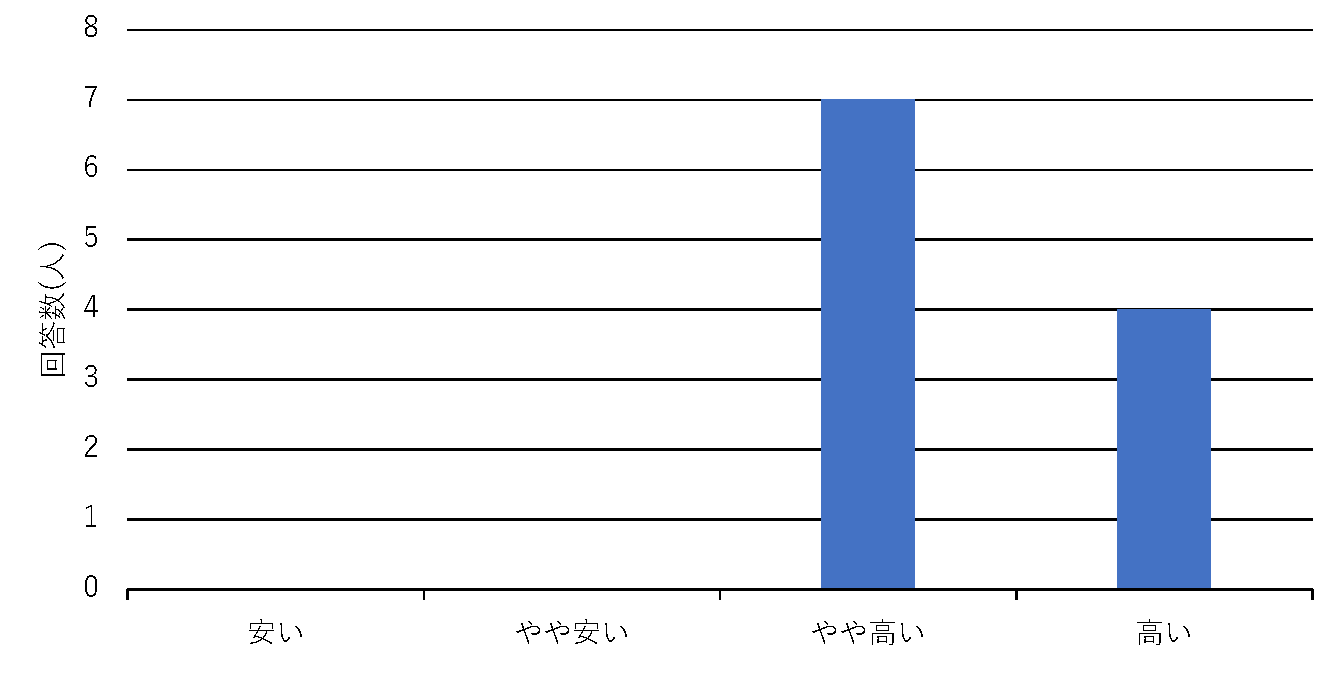
\includegraphics[clip,height=55mm]{
 アンケート2_3_2.pdf}
\end{center}
 \caption{質問3.2 VR機器は高価だと思いますか?}
 \label{fig:アンケート2_3_2.pdf}
\end{figure}

VR機器は何円くらいのもだと購入するかという質問の結果は図\ref{fig:アンケート2_3_3.pdf}に示す.
特になしという回答が多かった.
また選択した機材でほしいと思う機能として多かったのは,マップ機能であった.また次に多かったのは通話やメッセージの送信などのコミュニケーション機能である.

\begin{figure}[h]
\begin{center}
 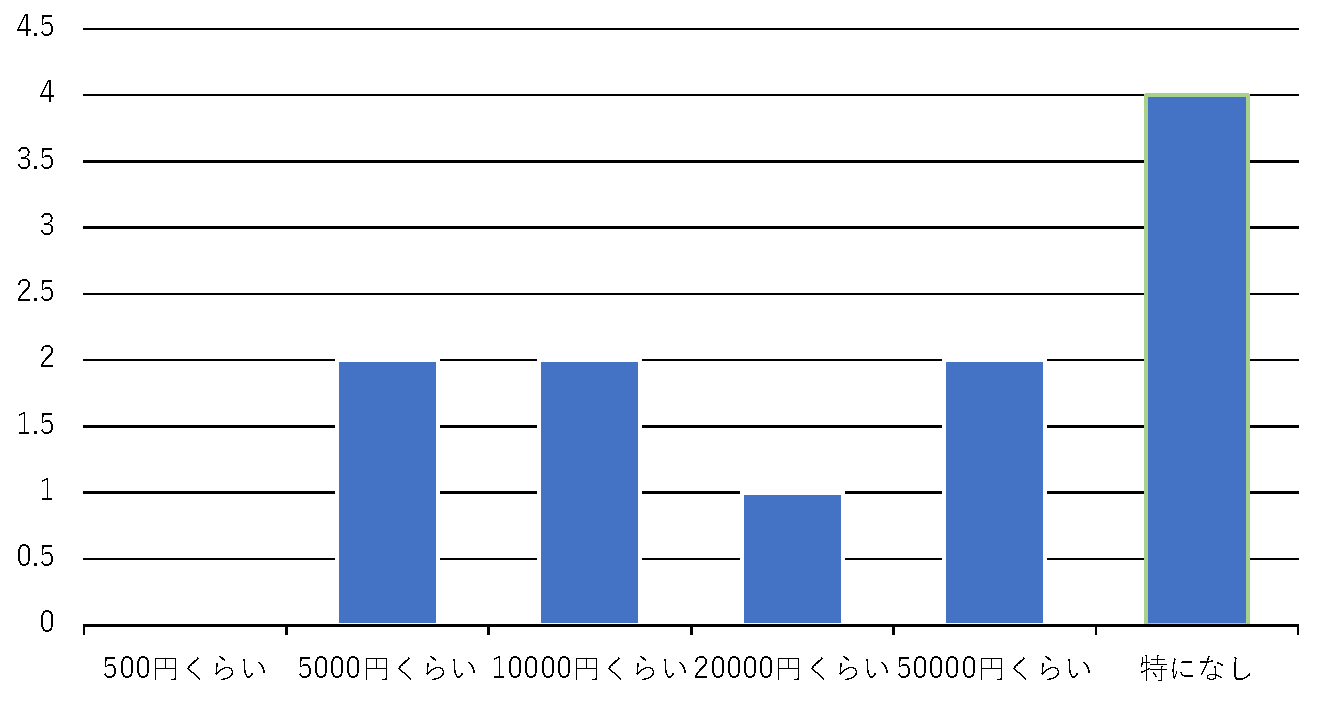
\includegraphics[clip,height=55mm]{
 アンケート2_3_3.pdf}
\end{center}
 \caption{質問3.3 VR機器は何円くらいのものだと購入を考えますか?}
 \label{fig:アンケート2_3_3.pdf}
\end{figure}

VR機器に対する印象は何かという質問の結果は図\ref{fig:アンケート2_3_5.pdf}に示す.
最も多かったのは高いというものだった.
次に多かったのは,体調不良になるというイメージだった.

\begin{figure}[h]
\begin{center}
 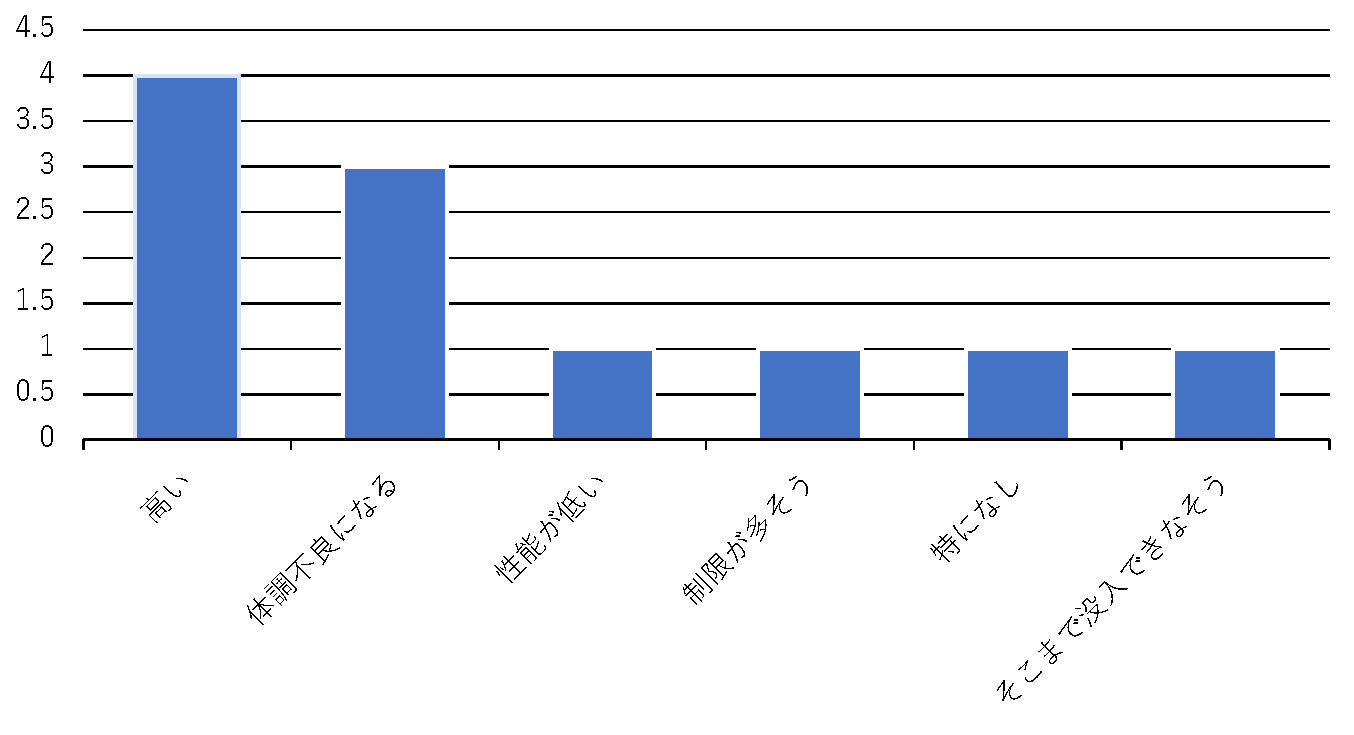
\includegraphics[clip,height=55mm]{
 アンケート2_3_5.pdf}
\end{center}
 \caption{質問3.5 VR機器に対する印象を教えてください}
 \label{fig:アンケート2_3_5.pdf}
\end{figure}

VR機器のお勧め度はどのくらいかという質問の結果は図\ref{fig:アンケート2_3_6.pdf}に示す.
全体的にはあまり勧めたいと思わない人が多いという結果になった.
その理由として多かった意見は,自分があまり興味がないからという意見だった.

\begin{figure}[h]
\begin{center}
 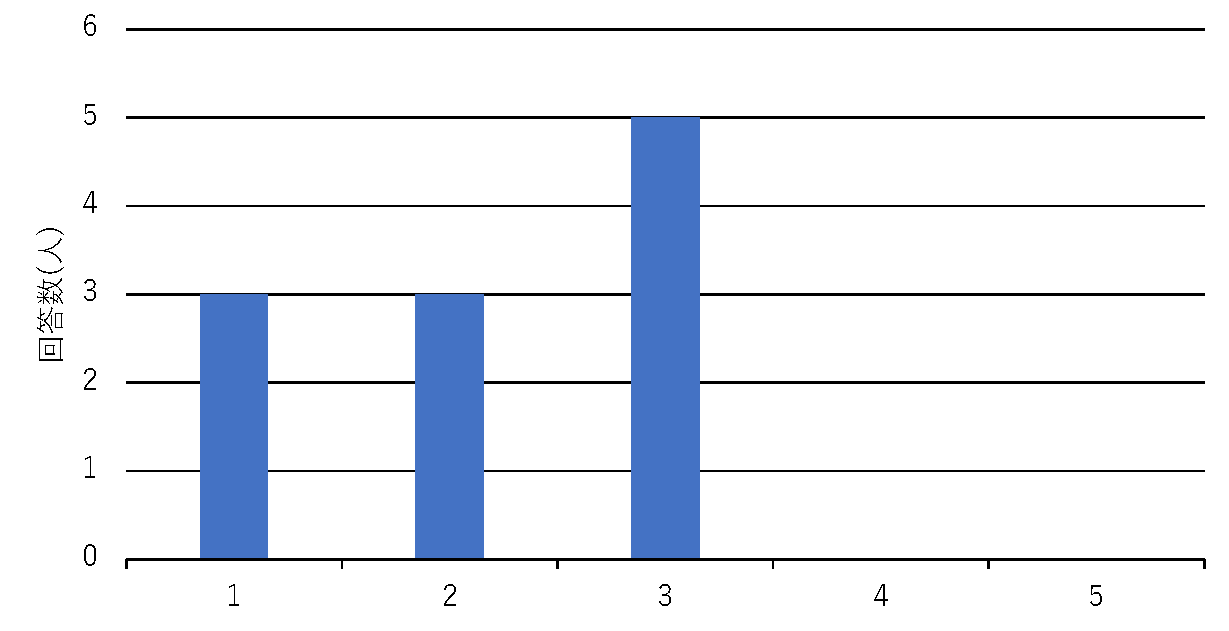
\includegraphics[clip,height=55mm]{
 アンケート2_3_6.pdf}
\end{center}
 \caption{質問3.6 VR機器を友人に勧める場合お勧め度はどのくらいですか?}
 \label{fig:アンケート2_3_6.pdf}
\end{figure}

\subsubsection{VRコンテンツに関する質問}
この質問は対象者69人全員が回答した.

VR機器を所持したらどのようなコンテンツを利用したいかという質問の結果は図\ref{fig:アンケート2_4_1.pdf}に示す.
最も多かったのはアクションコンテンツであった.
その次に多かったのはジェットコースターなどのアトラクションのコンテンツであった.

\begin{figure}[h]
\begin{center}
 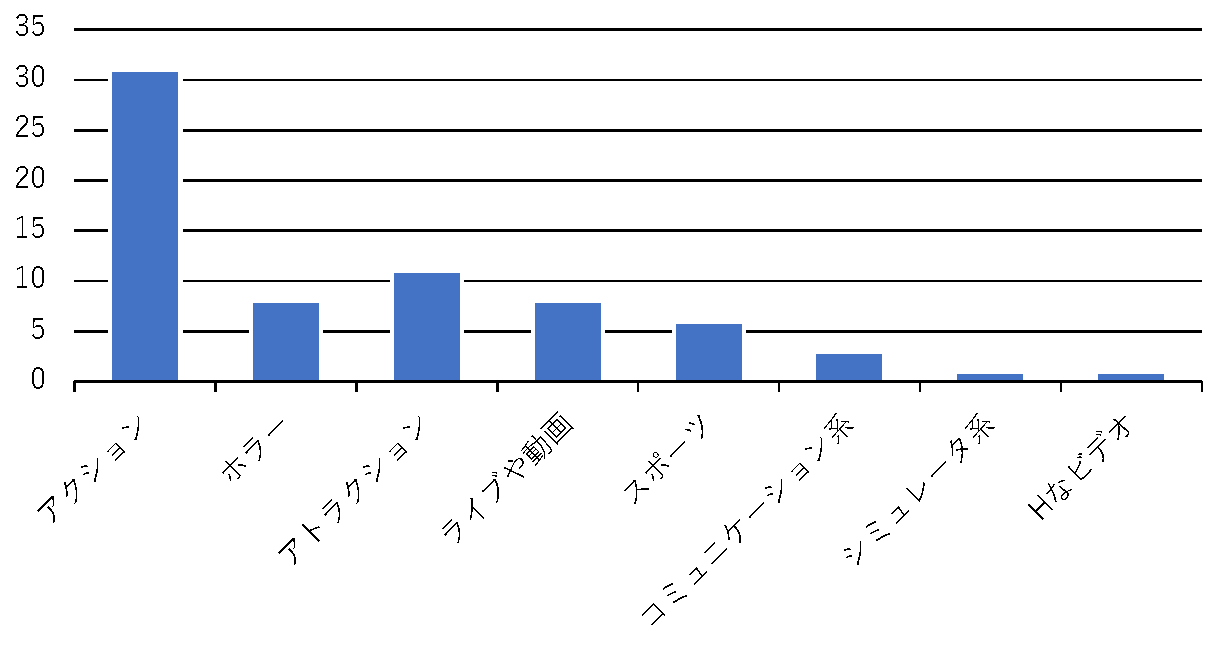
\includegraphics[clip,height=55mm]{
 アンケート2_4_1.pdf}
\end{center}
 \caption{質問4.1 VR機器を所持したとしたらどのようなコンテンツを1番利用したいですか?}
 \label{fig:アンケート2_4_1.pdf}
\end{figure}

各コンテンツでの購入意欲の調査結果は図\ref{fig:アンケート2_4_2.pdf}から図\ref{fig:アンケート2_4_5.pdf}に示す.

\begin{figure}[h]
\begin{center}
 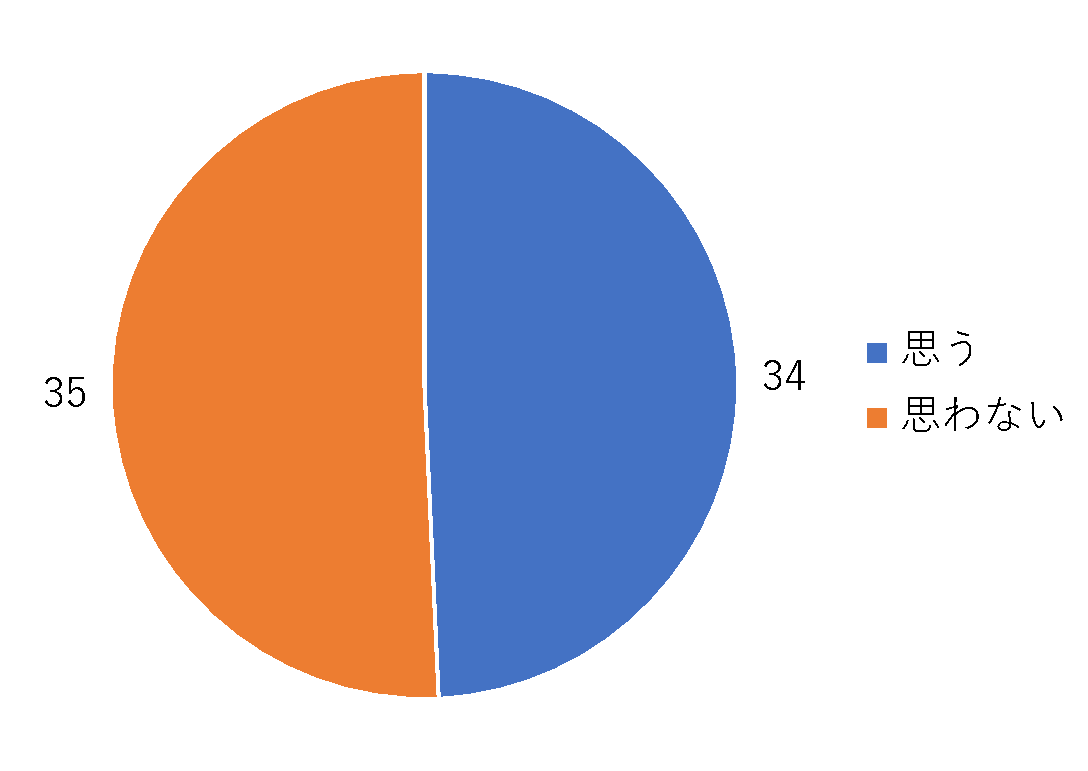
\includegraphics[clip,height=55mm]{
 アンケート2_4_2.pdf}
\end{center}
 \caption{質問4.2 VR空間で剣と魔法で戦うアクションを行うことができる本格的MMORPGのゲームがあります。
このゲームをプレイするためにVR機器を購入しようと思いますか?}
 \label{fig:アンケート2_4_2.pdf}
\end{figure}

\begin{figure}[h]
\begin{center}
 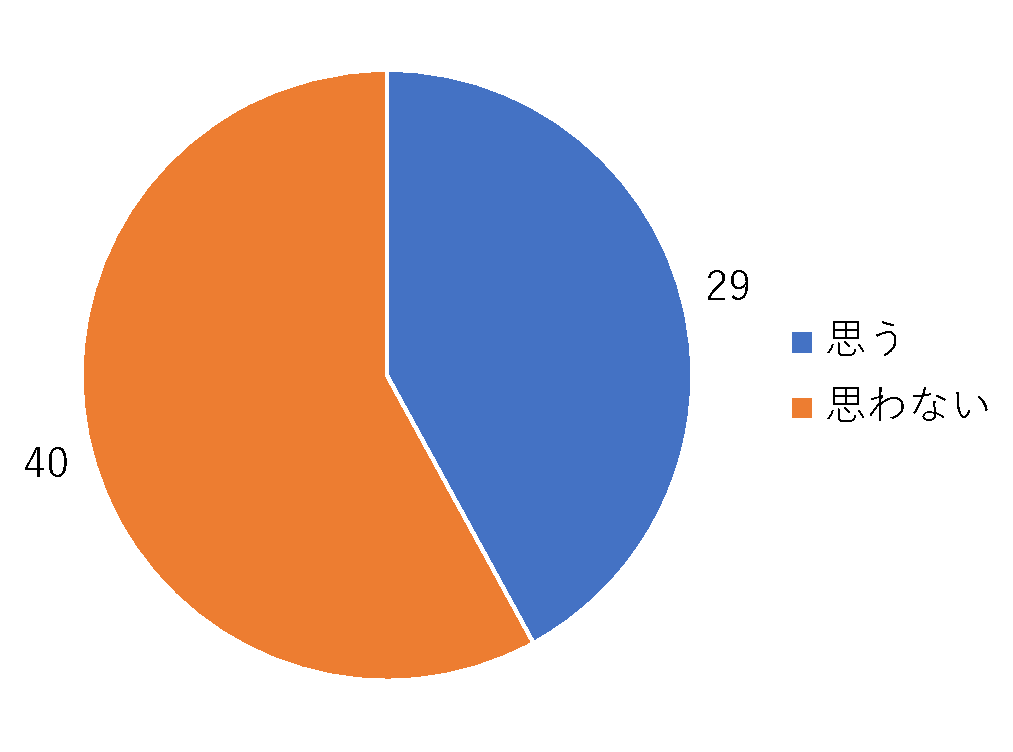
\includegraphics[clip,height=55mm]{
 アンケート2_4_3.pdf}
\end{center}
 \caption{質問4.3 アフェクテッド 恐怖の館というお化け屋敷的な体験型ホラーゲームがあります。多くのホラーシーンがあり、分岐ルートも存在するためたくさん楽しむことができます。
このゲームをするためにVR機器を購入しようと思いますか?}
 \label{fig:アンケート2_4_3.pdf}
\end{figure}

\begin{figure}[h]
\begin{center}
 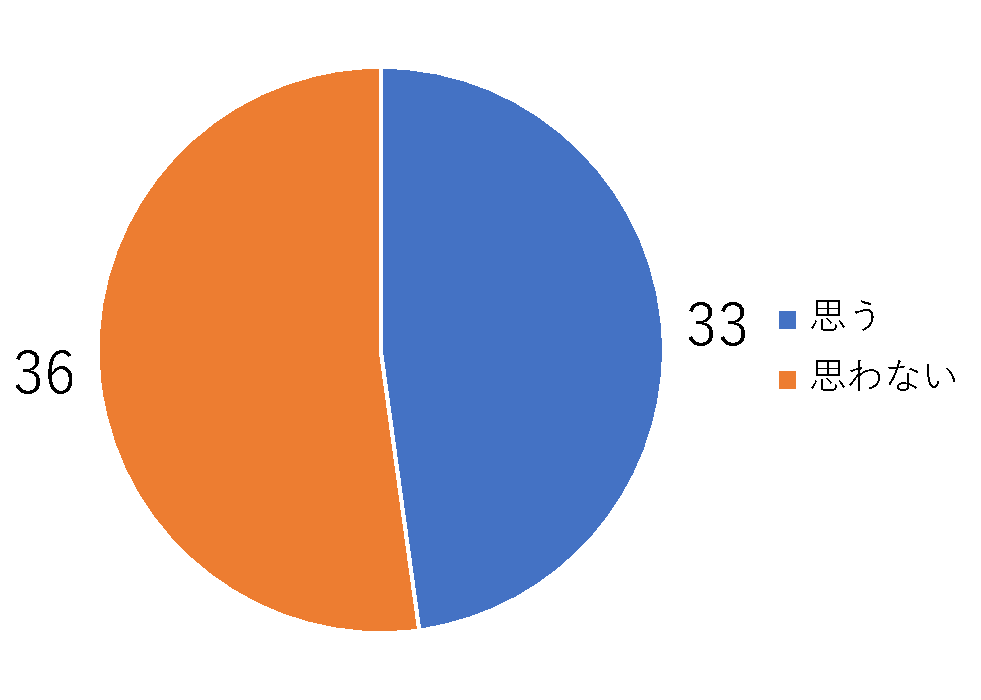
\includegraphics[clip,height=55mm]{
 アンケート2_4_4.pdf}
\end{center}
 \caption{質問4.4 アクションホラーゲームであるバイオハザード4のVRゲームがあります。このゲームは、手の動きによって武器を出し入れしてたたく使用になっています。
このゲームをするためにVR機器を購入しようと思いますか?}
 \label{fig:アンケート2_4_4.pdf}
\end{figure}

\begin{figure}[h]
\begin{center}
 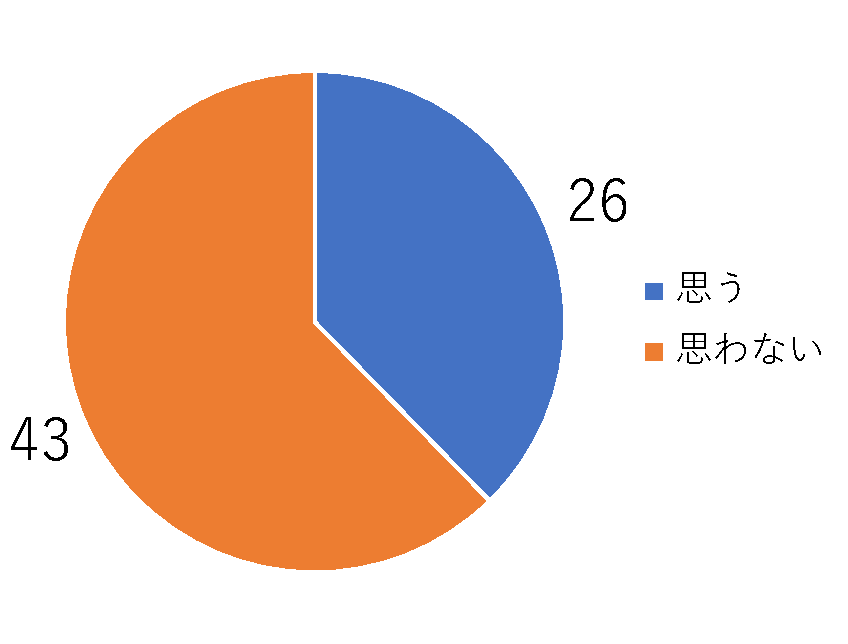
\includegraphics[clip,height=55mm]{
 アンケート2_4_5.pdf}
\end{center}
 \caption{質問4.5 宇宙船を舞台にした人狼ゲームである Among UsのVR版があります。宇宙船のクルーになり、間明込んでいる裏切り者を見つけ出すマルチプレイゲームです。
このゲームをするためにVR機器を購入しようと思いますか?}
 \label{fig:アンケート2_4_5.pdf}
\end{figure}

4つのコンテンツの中で最も購入したいコンテンツは何かという質問は,最も多かったのはZenith: The Last Cityというコンテンツであった.
理由としてゲームの世界に行った気分になる,アクションVRゲームが面白そうだからという意見が多かった.
次に多かったのは,Among Us VRだった.
理由としてやったことあるゲームだから,知っているゲームだからVRが分かりそうなどといった意見があった.

\begin{figure}[h]
\begin{center}
 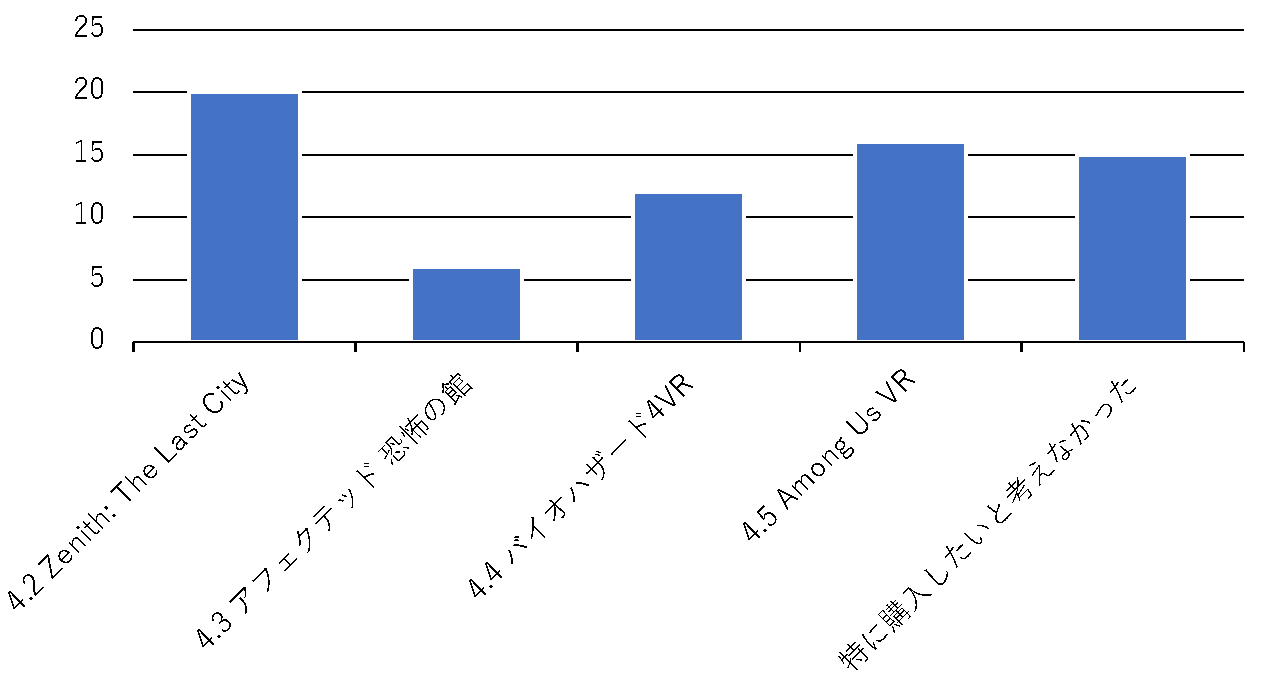
\includegraphics[clip,height=55mm]{
 アンケート2_4_6.pdf}
\end{center}
 \caption{質問4.6 4.2~4.5のうちどの質問で最も購入したいと考えましたか?}
 \label{fig:アンケート2_4_6.pdf}
\end{figure}


\clearpage

\section{考察}
\subsubsection{1回目のアンケートの考察}
最初に1回目のアンケートについて考察をしていく.

1回目のアンケートは,VR技術があまり利用されていない原因としてコンテンツ面に問題があるのではないかと仮説を立てて作成している.
1回目のアンケートに答えた123人のうち80人がVR体験をしたことがないと答えていたため,そもそもVRについての理解があまりないのではないかと考えた.
VRについての理解があまりないため分からないものを購入したいとは考える人は少ないだろう.
また,VRを体験したことがないと答えた80人のうち70人は機会がなかったためVR体験をしてこなかったと答えている.
そこからVRはより多くの人に気軽に体験ができる場所や機会を増やすと今よりも普及されるのではないかと考えた.

VR機材所持しているもしくは所持していた15人のうち12人は現在は利用していないと答えている.
その理由としてコンテンツに飽きたまたはやりたいコンテンツがないという意見よりも,機材が重たいや性能に満足していない,使うスペースがないといった機材面での意見が多かった.
しかしVR機器を実際に所持して利用した人の中で購入を勧めたいという人が10人いたことからVR技術というもの自体にはあまり不満はないと考えた.
また,VR機材を所持したことがない108人のうち85人が所持するまでに至らなかった理由として高価だからと答えている.
次に多い意見が利用する場所がないと答えている.
ここから現在のVRはコンテンツ面での問題よりも機材面での問題が多いと考えた.

1回目のアンケートでは,回答者全員に求めているコンテンツを質問したところ,アクションゲームやホラー体験,現実にある事象の体験,非現実的な体験,コミュニケーション系のコンテンツなどといったコンテンツが求めていると答えていた.
現在,アンケートの回答者が求めているコンテンツは多く存在しているがそのことを知らない人が多いのではないかと考えた.
また機材が普及しにくい理由として機材が重いことや広いスペースが必要,機材が高価ということから機材面に大きな問題があると考えた.
1回目のアンケートで,コンテンツ面ではあまり問題はなくVRを体験する場所と機会がないことと機材面に問題があることが分かった.

\subsubsection{2回目のアンケートの考察}
次に2回目のアンケートについて考察をしていく.

値段によってはVR機器の購入を勧める58人のうち機能と価格を見た中でお勧めするのによいと考えたものは,6万円の価格帯で本体のみで利用できるスタンドアローン型だがPCにも接続ができPCに接続することでPC向けのVRコンテンツを利用できる機材だった.
その理由として多かったのは,PCに接続ができるため汎用性が高そうという意見が多かった.
他にも3万円でスタンドアローン型の機材が好まれる傾向にあった.
また,22万円する機材は価格が高すぎるためお勧めしたいと考える人が少なく,7000円以下の機材だとスマートフォンを用いてVR技術を利用するためスートフォンの性能に依存するまたはスマートフォンの性能では不十分と考える人が多かったためお勧めする人は少なかった.
ここからVR機材に求められている性能として求められているのは,最低限の機能としてスタンドアローン型ということとスマートフォン以上の性能ということだと考えた.
また,より多くの人に求められるためにはPCに接続もできるといった汎用性の高さが求められる.

VR機器はどんな値段でも購入をおすすめしないと答えた11人は,主にVR機器に対して高価という印象と体調不良という印象が強いという結果が分かったことから主に興味のない人にはマイナスのイメージが強いのではないかと考えた.

コンテンツでは,図\ref{fig:アンケート2_4_6.pdf}から人とコミュニケーションが取るゲームかつVR専用のものの方が求められやすいと考えた.
アンケート結果で多く票をとれたコンテンツの意見として,VR感を楽しめそうという意見やコミュニケーションをとるのが楽しそうという意見が多かった.
このことから多くの人はVRアバターなどを使ったVRらしいと感じやすいコンテンツかつ人と関わりが多いものを求められやすいと考えた.
しかし,類似コンテンツとしてVRChatなどがすでに存在しているため,現状では新しいコンテンツはあまり必要ではない.

2回目のアンケートの結果から,VRという概念を感じやすくかつコミュニケーションが取れるコンテンツがありVR機器が今よりも安価でスマートフォン以上の性能になり気軽に体験できる施設が増えると利用者が増えると考えた.

\clearpage

\section{結言}
本研究では,VRの利用状況を調査するために2回のアンケートを実施した.
現状VRは,求められているコンテンツとしてコミュニケーションがとれるVRらしさを感じるという要素が必要だということが分かった.
しかしこの要素があるコンテンツは既に存在している.
また少数意見であった求められているコンテンツも近しいものはあるためコンテンツ面は現状で十分であることが分かった.

VRには,現在よりも安価な機材でスマートフォンの性能以上のものと気軽に体験できる機会が必要だということが分かった.
現在は数万円で買えた機材は過去には数百万円という値段だったが,スマートフォンなどに使われる安価なパーツや構造の単純化により現在の価格になったことから将来的には現在高価だと考えられている機材は安くなっていくと考えた\cite{VR機材が安価になった理由}.
技術の進歩がされて現在よりも安価な素材で性能が高まることが一般的に普及するためには必要であるだろう.

\clearpage

\section{謝辞}
本論文の執筆にあたり多くの方々にご協力いただきました.

指導教官である須田准教授には,いつも丁寧な指導と適切な助言をいただきました.
深く感謝いたします.

千葉工業大学情報科学部情報ネットワーク科の学生の皆様にはアンケート調査にご協力いただきました.感謝いたします.

最後に,本論文を執筆するにあたり協力してくださった全ての方に厚く御礼申し上げます.

\clearpage
\begin{thebibliography}{99}
\bibitem{VR}  ``流行体感から読み解くサービス未来予測 流行予想シリーズ ~VR(バーチャルリアリティ)編~'', https://research-platform.line.me/archives/38203466.html, 2022/9/2参照

\bibitem{VRの概念の登場}  ``VRはいつから普及が始まった?仮想現実の歴史を紐解く'', https://onetech.jp/blog/when-did-vr-become-popular-11526\#VR20, 2023/1/2参照

\bibitem{VRの初の商用化}  ``VRの初商用化は30年前、現代を生きるクリエイターが知っておくべき歴史と必要な視点とは'', https://creatorzine.jp/article/detail/538, 2023/1/2参照

\bibitem{ARとは}  ``AR(拡張現実)とは? 4つの種類とVR・MRとの違いを解説'', https://www.japancv.co.jp/column/4190/, 2023/1/6参照

\bibitem{ARの歴史}  ``AR100年史 |現実を拡張するテクノロジーの誕生と成長を紐解く'', https://note.com/hato\_fun/n/n4ca0e20000cb, 2023/1/6参照

\bibitem{MRとは}  ``MRとは? AR,VRとの違いやビジネスへの活用法を解説'', https://www.digital-transformation-real.com/blog/what-is-mr\#toc-0, 2023/1/6参照

\bibitem{MRの歴史1}  ``複合現実感の歴史と今後の展望'', https://www.jstage.jst.go.jp/article/isciesci/64/9/64\_343/\_pdf, 2023/1/6参照

\bibitem{MRの歴史2}  ``MR(Mixed Reality)が産業にもたらす可能性と未来―MRの利活用に向けて'', https://www.pwc.com/jp/ja/knowledge/column/disruptive-technology-insights/disruptive-technology-insight10.html, 2023/1/6参照

\bibitem{VRの機材}  ``VRの歴史が一目で分かるインフォグラフィック'', https://www.moguravr.com/vr-history-infographic/, 2023/1/6参照

\bibitem{グラス型ARデバイス}  ``注目が高まる「スマートグラス」とは? メガネ型デバイスがつくる近未来の生活'', https://www.nomura.co.jp/el\_borde/article/0051/, 2023/1/8参照

\bibitem{VR機材が安価になった理由}  ``VRハードウェアの基礎知識。歴史や仕組み、3大VR HMDの比較まで
'', https://www.watch.impress.co.jp/headline/docs/extra/vr/1060434.html, 2023/1/13参照

\end{thebibliography}

\end{document}
